% require
\documentclass[30pt]{article}
\usepackage{listings}
\usepackage{amsmath}
\usepackage[dvipsnames]{xcolor}  % for color
\usepackage{xcolor}


\usepackage{amsmath}
\usepackage{amsfonts}
\usepackage{tabularx}
\usepackage{listings}
\usepackage{hyperref} % for link
\usepackage[utf8]{inputenc}
\usepackage{tikz}
\usepackage{pdfpages}
\usepackage{fancyhdr}
\usepackage[margin=1.5cm]{geometry}
\usepackage{float}
\usepackage{graphicx,wrapfig,lipsum}
\usepackage{ptext}
% \usepackage{xepersian}
\setlength{\headsep}{1cm}
% \settextfont{Yas.ttf}


% end require

\lstdefinestyle{customc}{
  belowcaptionskip=1\baselineskip,
  breaklines=true,
  frame=L,
  xleftmargin=\parindent,
  language=python,
  showstringspaces=false,
  basicstyle=\footnotesize\ttfamily,
  keywordstyle=\bfseries\color{green!40!black},
  commentstyle=\itshape\color{purple!40!black},
  identifierstyle=\color{blue},
  stringstyle=\color{orange},
}

% \lstset{
%     language=Python,
%     basicstyle=\ttfamily\small,
%     keywordstyle=\color{blue},
%     stringstyle=\color{red},
%     commentstyle=\color{green},
%     morecomment=[l][\color{magenta}]{\#},
%     frame=single,
%     breaklines=true,
%     postbreak=\mbox{\textcolor{red}{$\hookrightarrow$}\space},
% }

% \lstset{escapechar=@,style=customc}

\lstdefinestyle{mystyle}{
    backgroundcolor=\color{gray!10},   
    commentstyle=\color{green!40!black},
    keywordstyle=\color{blue},
    numberstyle=\tiny\color{gray},
    stringstyle=\color{orange},
    basicstyle=\footnotesize\ttfamily,
    breakatwhitespace=false,         
    breaklines=true,                 
    captionpos=b,        
    language = python,
    keepspaces=true,                 
    numbers=left,                    
    numbersep=5pt,                  
    showspaces=false,                
    showstringspaces=false,
    showtabs=false,                  
    tabsize=2,
    frame=single
}




\lstset{style=mystyle}

\begin{document}
% var
\newcommand{\master}{Dr. Yassaee}
\newcommand{\lesson}{Probability and Statistics}
\newcommand{\name}{Mohammad Mohammadian, Ali Torkaman}
\newcommand{\detail}{Project Report}
\newcommand{\subject}{Introduction to random walk}
% end var

% page first %
\begin{center}
\tikz[remember picture,overlay] \node[opacity=0.3,inner sep=0pt] at (current page.center){
\includegraphics[width=\paperwidth,height=\paperheight]{pic/logo/bg1.jpg}};

In The Name Of God \\
{\fontsize{35}{20} \selectfont \lesson} \\
{\huge \master}
\vspace{1cm}
\begin{figure}[H]
    \centering
    
\includegraphics[scale = 0.75]{pic/logo/sharif.png}
\end{figure}
\vspace{3cm}

{\large	\name}\\
\vspace{1.5cm}
{\large \detail}\\
{\large \subject}\\
\vspace{.5cm}
{\large \today}
\end{center}
\thispagestyle{empty}
\newpage
% end page first

% header first and first page
{\Huge  \lesson}\\
{\LARGE \name}\\
{\large \detail : \subject }
\hfill%
%\begin{minipage}{0.01\textwidth}

\includegraphics[width=2cm]{pic/logo/sharif2.png}
%\end{minipage}
\vspace{0.5cm}
\hrule
\vspace{0.5cm}
% end header

In this paper we explain our project and what we done in it. Explain our solutions to theory problems! 
\begin{figure}[h]
\centering
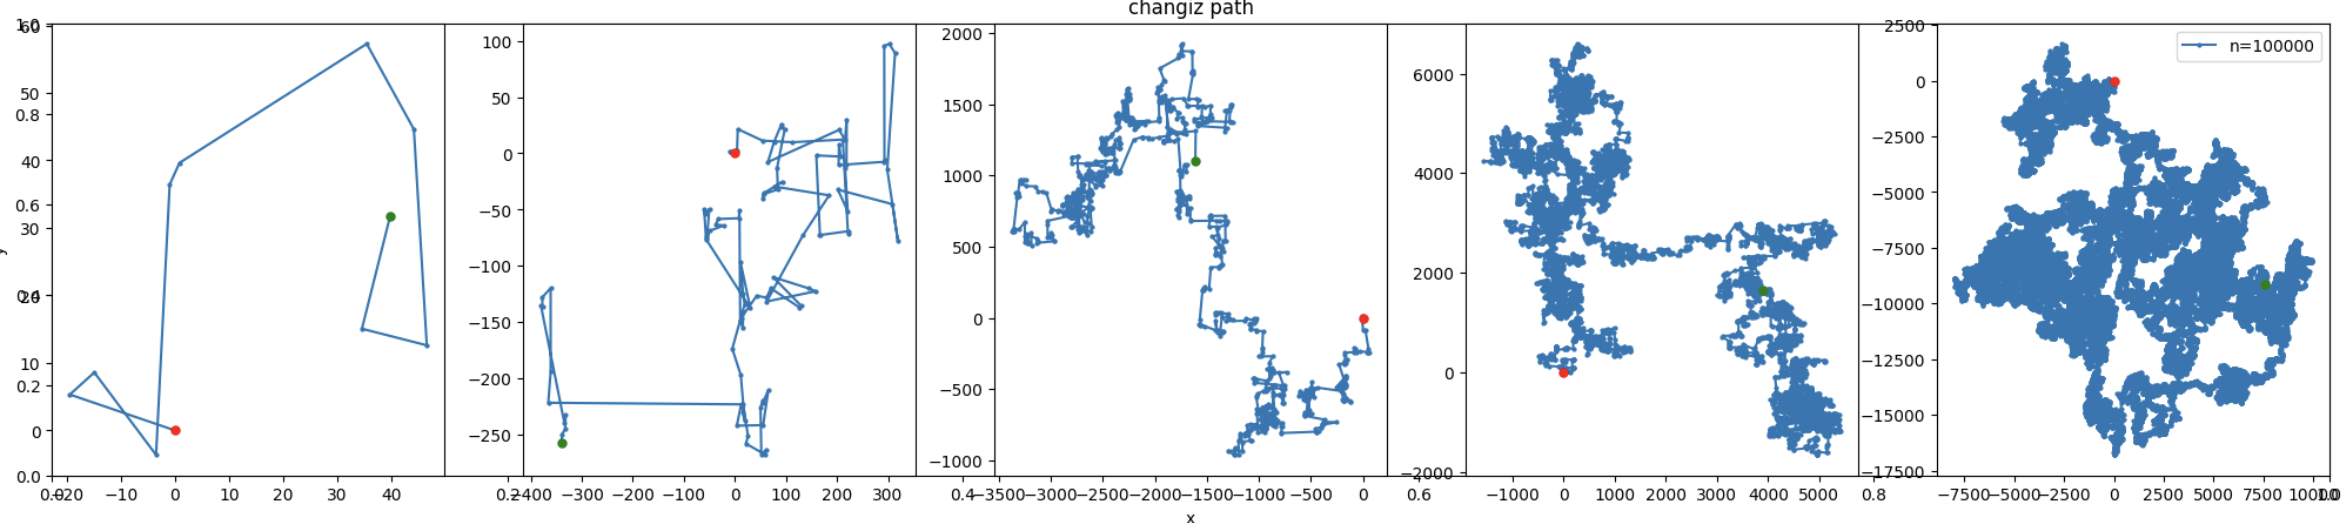
\includegraphics[width=500,height = 160]{pic/fig/prob_Project-1.png}
\end{figure}
\begin{figure}[h]
\centering
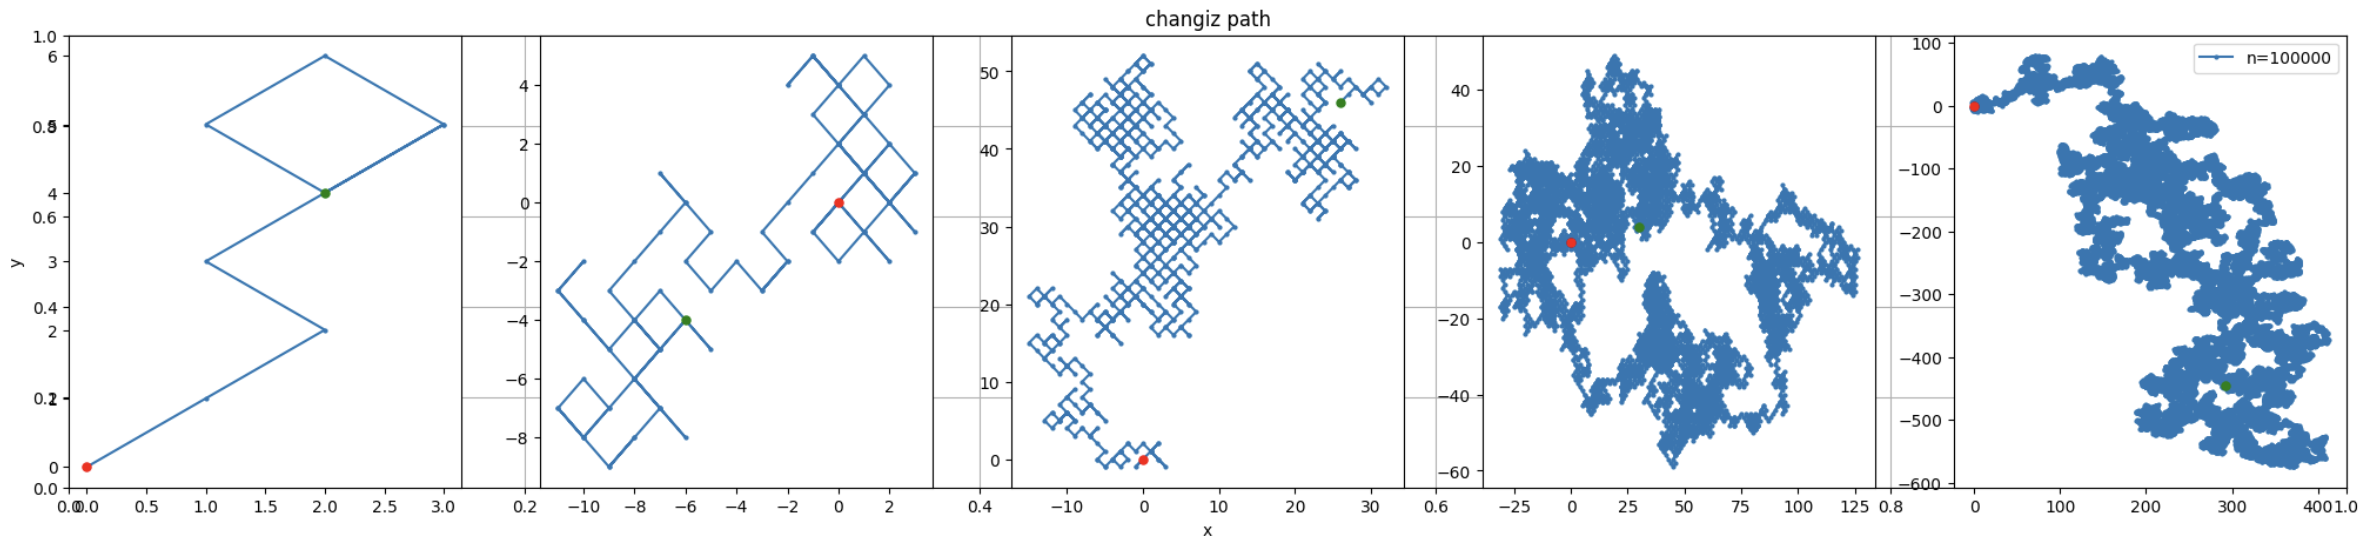
\includegraphics[width=500,height = 160]{pic/fig/prob_Project-2.png}
\end{figure}
\begin{wrapfigure}{r}{0.25\textwidth} %this figure will be at the right
    \centering
    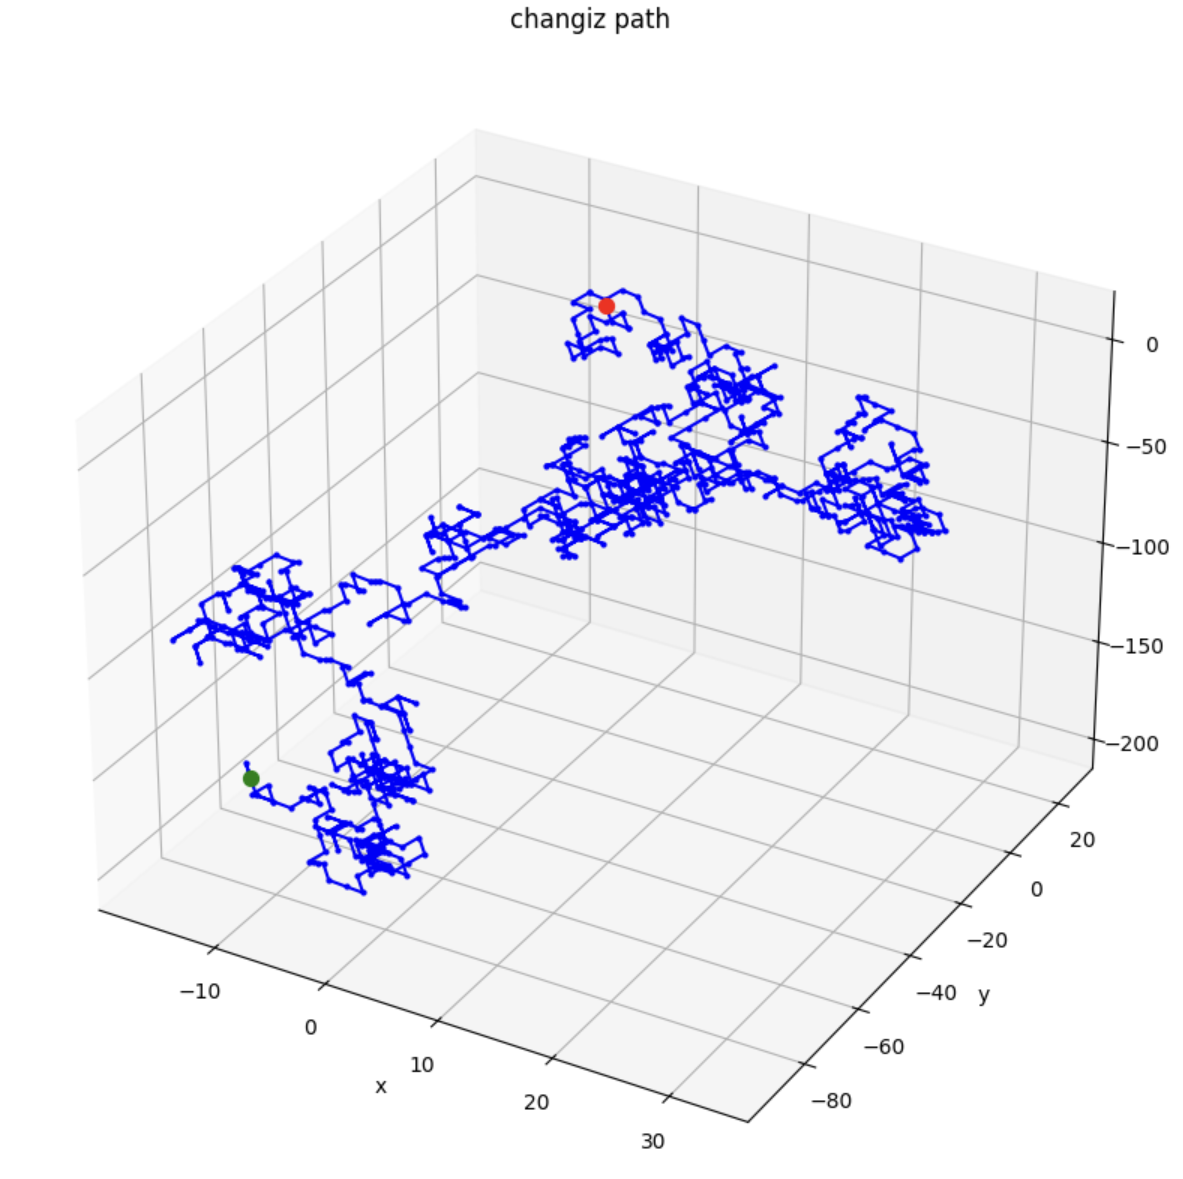
\includegraphics[width=170,height = 170]{pic/fig/prob_Project-3.png}
\end{wrapfigure}
Here's some outputs for CHWs of Project. 
\newpage
% header and footer
\pagestyle{fancy}
\chead{{\large \lesson}}
\lhead{\detail}
\rhead{\master}
\rfoot{\name}
\lfoot{{\subject}}
\cfoot{\thepage}
\renewcommand{\footrulewidth}{1pt}
% end header and footer


{\Large \color{blue} Theory 1 (Markov's inequality)} \\
{\color{blue} Let X be a continuous random variable with positive values and $a > 0$ . In this case we have:
\begin{center}
    
    $\Bbb{P}[X \ge a] \le \frac{\Bbb{E}[X]}{a} $
\end{center} \\
}
{\color{black} 
We have : \\
\begin{center}
    $\Bbb{E}[X] = \int_{-\infty}^{\infty}{xf_X(x)dx} $  \vspace{0.5cm}\\
    $= \int_{0}^{\infty}{xf_X(x)dx}$  \hspace{1cm}  (since X is positive valued) \vspace{0.25cm}\\
    $\ge \int_{a}^{\infty}{xf_X(x)dx} $ \hspace{1cm} (for any $a \ge 0$ ) \vspace{0.25cm}\\
    $\ge \int_{a}^{\infty}{af_X(x)dx} $ \hspace{1cm} (since $x \ge a$ in the integrated region) \vspace{0.5cm}\\
    $= a \int_{a}^{\infty}{f_X(x)dx}$ \vspace{0.25cm}\\
    $ = a\Bbb{P}[X \ge a] $
\end{center} \\
So we have : \\
\begin{center}
    $\Bbb{E}[X] \ge a\Bbb{P}[X \ge a] \Rightarrow \Bbb{P}[X \ge a] \le \frac{\Bbb{E}[X]}{a} $
\end{center} \\
}
{\Large \color{blue} Theory 2 } \\
{\color{blue} Changiz has a high skill in hacking and infiltrating information systems. By hacking the city's subway information, he gets access to the origin and destination of all passengers and extracts the passengers' information. Analyzing this information, he realizes that the percentage of people who get off at the "Circus" station in one day can be modeled with a random variable with a mean of 75 and a variance of 25. Also, he found that random variables related to different days are independent from each other. \\ } \newline
{\color{blue}{\large  1.} Find an upper bound for the probability that tomorrow at least 85 \% of the people will get off at the circus station.} \\

We use Markov's inequality and define $a = 85$ : \\
\begin{center}
    $\Bbb{P}[X > 85] \le \frac{\Bbb{E}[X]}{85} = \frac{75}{85} = \frac{15}{17} $
\end{center} \\

{\color{blue}{\large  2.} Find a lower bound for the probability that between 65\% and 85\% of people will get off at the circus station tomorrow. } \\


In this case we define a new random variable $Y = (X - \Bbb{E}[X])^2 $ . We know that $\Bbb{E}[Y] = 25 $ .\\
The problem asks us to find a lower bound for $\Bbb{P}[Y < 100] $ . We use Markov's inequality in this case too : \\

\begin{center}
    \Bbb{P}[Y > 100] \le \frac{\Bbb{E}[Y]}{100} = \frac{25}{100} = \frac{1}{4} \vspace{0.25cm}\\
    $\rightarrow \Bbb{P}[Y > 100] = 1 - \Bbb{P}[Y < 100] $ \vspace{0.25cm}\\
    $\Rightarrow 1 - \Bbb{P}[Y < 100]  \le \frac{1}{4} $ \vspace{0.25cm}\\
    $\Rightarrow \frac{3}{4} \le \Bbb{P}[Y < 100] $
\end{center} \\
We could use Chebyshev's inequality directly too. 

\newpage
{\color{blue}{\large  3.} How many days should we check the information to make sure that with a probability of at least 0.90, the average percentage of people who got off at the circus station during these days was between 70 and 80 percent? } \\
With Chebyshev's inequality we have : \\
\begin{center}
    $\Bbb{P}(|\frac{\sum X_i}{n} - \mu | > \epsilon) \le \frac{\sigma^2}{n\epsilon^2} $ \vspace{0.25cm} \\
    $\Bbb{P}(|\frac{\sum X_i}{n} - \mu | > \epsilon) = 1 - \Bbb{P}(|\frac{\sum X_i}{n} - \mu | \le \epsilon) = 1 - 0.9 = 0.1 $ \vspace{0.25cm} \\
    $n \le \frac{\sigma^2}{\epsilon^2 \Bbb{P}(|\frac{\sum X_i}{n} - \mu | > \epsilon)} = \frac{0.25^2}{0.05^2 \times 0.1} = 250 $
\end{center}

{\Large \color{blue} Theory 3 } \\
{\color{blue} Changiz has also gained access to the information of subway trains. He found out that the number of trains that pass by the station near his house in a period of time τ can be modeled with the help of a random variable X which is $X \sim Poisson(\lambda)$. He also found out that the number of trains in time intervals which do not share with each other, are independent of each other. \\ } \newline
{\color{blue}{\large  1.} We define the random variable $Z_n$ as the number of trains that have passed by the station near Changiz House in the time period $T = n\tau$ . Suppose $k > 1$ . Find an upper bound for the following expression: } \\ \newline
The time $n\tau$ can be separate to $n$ intervals of size $\tau$ . So the number of trains in this time is a random variable $Z_n \sim Poisson(n\lambda)$. Because it's n times sum of $X \sim Poisson(\lambda)$ and we know that the sum of tow poisson random variables has a poisson distribution with $\lambda_1 + \lambda_2 $ . Now we use Markov's inequality : \\
\begin{center}
    $\Bbb{P}[Z_n \ge kn\lambda] \le \frac{\Bbb{E}[Z_n]}{kn\lambda} = \frac{\lambda n}{kn\lambda} = \frac{1}{k}$ \vspace{0.25cm} \\
    $\Rightarrow \Bbb{P}[Z_n \ge kn\lambda]  \le \frac{1}{k}$
\end{center} \\ \newline
{\color{blue}{\large  2.} Suppose $k = 1.25$ , $n = 20$ , $\lambda = 1 $. Estimate the Central Limit Theorem of the previous part with the help of a theorem. } \\ \newline
Like previous part we separate the intervals. suppose that the number of trains in i'th interval is a random variable $X_i$ . With CLT we have : \\ 
\begin{center}
    $\Bbb{P}(\frac{X_1+X_2+...+X_n - n\lambda}{\sqrt{n\lambda}} \le a ) = \Phi(a) $
\end{center} \\
Now we have to find the 'a' : \\
\begin{center}
    $\Bbb{P}(X_1+X_2+...+X_n - n\lambda \le a\sqrt{n\lambda} ) $ \vspace{0.25cm} \\
    $\Bbb{P}(X_1+X_2+...+X_n \le a\sqrt{n\lambda} + n\lambda ) =\Bbb{P}(Z_n \le a\sqrt{n\lambda} + n\lambda )$ \vspace{0.25cm} \\
    $\rightarrow a\sqrt{n\lambda} + n\lambda  = kn\lambda \Rightarrow a = (k-1)\sqrt{n\lambda} $ \vspace{0.25cm} \\
\end{center} \\
So for $a = (k-1)\sqrt{n\lambda} $ we have : \\ 
\begin{center}
    $1 - \Bbb{P}(Z_n \ge kn\lambda) = \Bbb{P}(\frac{X_1+X_2+...+X_n - n\lambda}{\sqrt{n\lambda}} \le a ) = \Phi(a)  $ \\
\end{center} \\
So we have : \\ 
\begin{center}
    $\Bbb{P}(Z_n \ge kn\lambda) = 1 - \Phi((k-1)\sqrt{n\lambda}) = 1 - \Phi(1.118) = 1 - 0.86822 \approx 0.131 $
\end{center} \\ \newline 

{\Large \color{blue} Theory 4 } \\
{\color{blue} We define $Z_n = \sum_{i=1}^{n}{X_i}$ where $X_i$'s are independent random variables with the same distribution. Prove that : \\
\begin{center}
    $\Psi_{Z_n}(s) = n \Psi_X(s) $
\end{center}
\\ } \newline
We have : \\
\begin{center}
    $\Phi_{Z_n}(s) = \Bbb{E}(e^{sX_1+sX_2+...+sX_n}) \Rightarrow $ Because they are independent $ \Rightarrow \prod_{i =1}^{n} \Bbb{E}(e^{sX_i}) $ \vspace{0.25cm}\\
    $\Rightarrow \Phi_{Z_n}(s) = \prod_{i =1}^{n} \Bbb{E}(e^{sX_i}) = \mathbb{E}(e^{sX_i})^n = \Phi_X(s)^n $ \vspace{0.25cm} \\
    $\Rightarrow \Psi_{Z_n} = n \Psi_X(s) $
\end{center} \\

{\Large \color{blue} Theory 5 } \\
{\color{blue} If we assume $s > 0 $ , $\beta > \Bbb{E}[X] $ . Prove that : \\
\begin{center}
    $ e^{-rn} \ge \Bbb{P}[e^{sZ_n} \ge e^{s\beta n}] = \Bbb{P}[Z_n \ge \beta n] $
\end{center} \\
Where $r = sup\{s\beta - \Psi_X(s)\} $ . 
\\ } \newline 
For the first part because $s \ge 0 $ we have : \\
\begin{center}
    $Z_n \ge \beta n \Longleftrightarrow sZ_n \ge s\beta n \Longleftrightarrow e^{sZ_n} \ge e^{s\beta n} $ \vspace{.25cm} \\
    So we have :  $ \Bbb{P}[e^{sZ_n} \ge e^{s\beta n}] = \Bbb{P}[Z_n \ge \beta n] $
\end{center} \\
For second part we use Markov's inequality : \\ 
\begin{center}
    $\Bbb{P}[e^{sZ_n} \ge e^{s\beta n}] \le \frac{\Bbb{E}[e^{sZ_n}]}{e^{s\beta n}} = (\frac{\Bbb{E}[e^{sX}]}{e^{s\beta}})^n = (\frac{\Phi_X(s)}{e^{s\beta }})^n $
\end{center} \\ 
Clearly we have to proof $\frac{\Phi_X(s)}{e^{s\beta }} \le e^{-r} $ : \\
\begin{center}
    $\Longleftrightarrow \frac{\Phi_X(s)}{e^{s\beta }} \le e^{-r} $ \hspace{.3cm} (For all $s \ge 0$) \vspace{.25cm} \\ 
    get ln : $\Rightarrow \Psi_X(s) - s\beta \le -r  $ \vspace{0.25cm} \\
    $ \Longleftrightarrow r \ge s\beta - \Psi_X(s) $
\end{center} \\
Last inequality holds because we have : \hspace{0.5cm} $r = sup\{s\beta - \Psi_X(s)\} $ \\ \newline

{\Large \color{blue} Theory 6 }  \vspace{0.2cm} \\
{\color{blue}{\large 1.} If we assume $X \sim normal(\mu,\sigma^2) $ . Find $\Psi_X(s) $ . } \\
We have : \\
\begin{center}
    $\Bbb{E}(e^{sX}) = M_X(s) = \Bbb{E}(e^{sX}) = \int_{-\infty}^{\infty}e^{sx}\frac{1}{\sigma\sqrt{2\pi}}e^{-\frac{1}{2}(\frac{x-\mu}{\sigma})^2}dx $ \vspace{0.25cm} \\
    $= \frac{1}{\sigma\sqrt{2\pi}}\int_{-\infty}^{\infty}exp\{sx-\frac{1}{2}(\frac{x-\mu}{\sigma})^2\} dx $
\end{center}  \vspace{0.25cm} \\
Substituting $u = \frac{x - \mu}{\sqrt{2}\sigma} $ , we have $ x = \sqrt{2}\sigma u +\mu $ : \\
\begin{center}
    $M_X(s) = \frac{1}{\sqrt{\pi}} \int_{-\infty}^{\infty}exp\{(\sqrt{2}\sigma u +\mu)s - u^2 \} du $\vspace{0.25cm} \\
    $= \frac{e^{s\mu}}{\sqrt{\pi}} \int_{-\infty}^{\infty}exp\{- (u^2 - \sqrt{2}\sigma us )\} du $ \vspace{0.25cm} \\
    $= \frac{e^{s\mu}}{\sqrt{\pi}} \int_{-\infty}^{\infty}exp\{- (u - \frac{\sigma s}{\sqrt{2}})^2 + \frac{1}{2}\sigma^2s^2  \} du $ \vspace{0.25cm} \\
    $= \frac{exp\{s\mu + \frac{1}{2}\sigma^2s^2\}}{\sqrt{\pi}} \int_{-\infty}^{\infty}exp\{- (u - \frac{\sigma s}{\sqrt{2}})^2 \} du $
\end{center} \vspace{0.25cm} \\
Substituting $ v = u - \frac{\sigma s}{\sqrt{2}})^2 $ , clearly we have : \\
\begin{center}
    $M_X(s) = \frac{exp\{s\mu + \frac{1}{2}\sigma^2s^2\}}{\sqrt{\pi}} \int_{-\infty}^{\infty}exp(-v^2) dv $
\end{center} \vspace{0.25cm} \\
With the Gaussian integral we have : \hspace{1cm} $\int_{-\infty}^{\infty}e^{-x^2}dx = \sqrt{\pi} $ \vspace{0.25cm} \\
So we have : \\
\begin{center}
    $M_X(s) = \frac{exp\{s\mu + \frac{1}{2}\sigma^2s^2\}}{\sqrt{\pi}} \int_{-\infty}^{\infty}exp(-v^2) dv  = exp(s\mu + \frac{1}{2}\sigma^2s^2) $ \vspace{0.25cm} \\
    $\Rightarrow \Psi_X(s) = ln(\Bbb{E}[e^{sX}]) = ln(M_X(s)) = s\mu + \frac{1}{2}\sigma^2s^2 $
\end{center}

{\color{blue}{\large 2.} For each random variable X assuming $\Bbb{E}[X] = 0 $ and $|X| < M $ Show: \hspace{1cm} $\Psi_X(s) \le \frac{1}{2}M^2s^2 $ . } \\ 
We prove something stronger : \\
{\color{BrickRed}Lemma :  Suppose that $\Bbb{E}[X] = 0 $ and that $a \le X \le b$ . Then : \hspace{1cm} $\Bbb{E}(e^{sX}) \le e^{\frac{s^2(b-a)^2}{8}} $ } \vspace{0.5cm} \\

{\color{Maroon} Since $a \le X \le b$ , we can write $X$ as a convex combination of $a$ and $b$ , namely $X = \alpha b + (1 - \alpha )a$ where $\alpha = \frac{X - a}{b - a} $ . By convexity of the function $y \rightarrow e^{ys} $ we have : \\
\begin{center}
    $e^{sX} \le \alpha e^{sb} + (1 - \alpha)e^{sa} = \frac{X - a}{b - a}e^{sb} + \frac{b - X}{b-a}e^{sa} $
\end{center} \\
Take expectations of both sides and use the fact $\Bbb{E}[X] = 0 $ to get : \\
\begin{center}
     $e^{sX} \le \frac{ - a}{b - a}e^{sb} + \frac{b }{b-a}e^{sa} = e^{g(u)} $ \hspace{0.5cm} where $u = s(b - a) $
\end{center} \\
we have : $g(u) = -\gamma u + ln(1 - \gamma + \gamma e^u ) $ and $\gamma = \frac{-a}{b - a} $ . \\
Now note that $g(0) = g'(0) = 0 $ . Also $g''(u) \le \frac{1}{4}$ for all $u > 0 $ . \\
By Taylor's theorem , there is a  $\varepsilon \in (0,u) $  : \\
\begin{center}
    $g(u) = g(0) + ug'(0) + \frac{u^2}{2} g''(\varepsilon) = \frac{u^2}{2} g''(\varepsilon) \le \frac{1}{u^2} \times \frac{1}{4} = \frac{u^2}{8} = \frac{s^2(b-a)^2}{8} $ 
\end{center} \\
Finally we have : \\
\begin{center}
    $\Bbb{E}[e^{sX}] \le e^{g(u)} \le e^{\frac{s^2(b-a)^2}{8}} $
\end{center} } \\ 
Because we know that $-M \le X \le M $ taking $a = -M $ and $b = M$ the proof is done. \\ \newline
Another way is : \\ 
\begin{center}
    $1 = \Bbb{P}(|X| < M) = \Bbb{P}(X^2 < M^2) = \Bbb{P}(-X^2 > -M^2) =\Bbb{P}(-sX^2 > -sM^2)$  \vspace{0.3cm} \\
    $= \Bbb{P}(e^{-sX^2} > e^{-sM^2}) \le \frac{\Bbb{E}(e^{-sX^2})}{e^{-sM^2}} $
\end{center}

{\color{blue}{\large 3.} We define $Z_n = \sum_{i=1}^{n}{X_i}$ where $X_i$'s are independent random variables with the same distribution , and we know $ |X_i| \le M $ , $ \beta > \Bbb{E}[X] $ :\\
\begin{center}
    $\Bbb{P}[Z_n \ge \beta n] \le e^{-\frac{\beta ^ 2}{2M^2}n} $
\end{center}
} \\
We have : \\
\begin{center}
    $r = sup\{ s\beta - \Psi_x(s) \} \ge s\beta - \frac{M^2s^2}{2} = f(s)$
\end{center} 
Now we find the maximum of $f(s)$ : \hspace{0.3cm} $\frac{df}{ds} = 0 \rightarrow s = \frac{\beta}{M^2}$ \\
So we can get $r = \frac{\beta^2}{2M^2} $ in {\color{blue}Theory 5} : \\
\begin{center}
    $\Bbb{P}[Z_n \ge \beta n] \le e^{\frac{\beta^2}{2M^2}n} $
\end{center}

\newpage 
{\huge \color{blue} PART 3} \\ \newline
{\large \color{blue} First, we want to examine the random walk in one dimension and discover some of its basic properties together. A random walk in one dimension is a stochastic process like $\{Z_n\}_{n = 0}^{+\infty} $ : \\ 
\begin{center}
    $Z_n = Z_0 + \sum_{i = 0}^{n}X_i$
\end{center}
} \\ \newline 

{\Large \color{blue} Theory 7 } \\
{\color{blue} Changiz enters the subway station. The subway line where Changiz is located has an infinite number of stations, starting from number 1 and continuing to +∞. He decides to use a coin with probability p to ride the subway. He tosses the coin, if the result of the coin is a line, he does not get on the subway, and if the result is a lion, he gets on the subway and gets off at the next station. He repeats the same process independently at each station. Let $Z_n$ represent the number of Changiz station after $n$ coin toss. } \\ \newline
{\color{blue} {\large 1. } Find the probability mass function of the random variable $Z_n$ . } \\ \newline
We know he can't go back so if he is at station $Z_0$ at first , $\Bbb{P}[Z_n = k] = 0 $ for $k < Z_0 $ .For $k \ge Z_0 $ we have : \\ 
\begin{center}
    $\Bbb{P}[Z_n = k] = \begin{pmatrix} n \\ k-z_0 \end{pmatrix} p^{k - z_0}(1 - p)^{n - (k - z_0)}  $
\end{center} \newline
{\color{blue} {\large 2. } Find $\Bbb{E}[X_i] $ and Var$[X_i] $ . } \\ \newline
We have : \\
\begin{center}
    $X_i = 
    \begin{cases}
        1 & p \\
        0 & 1-p
    \end{cases}$
\end{center} \\
So $X_i \sim Bernoulli(p)$ and we have : \hspace{0.25cm} $\Bbb{E}[X_i] = p $ \hspace{0.25cm} Var$[X_i] = p(1-p) $  \\ \newline

{\color{blue} {\large 3. } Find $\Bbb{E}[Z_n] $ and Var$[Z_n] $ . } \\ \newline
We have : \\
\begin{center}
    $\Bbb{E}[Z_n] = \Bbb{E}[Z_0 + X_1 + X_2 + ... + X_n] = z_0 + n\Bbb{E}[X_i] = z_0 + np  $
\end{center} \\
For Var$[Z_n] $ first we calculate $\Bbb{E}[Z_n^2] $ : \\
\begin{center}
    $\Bbb{E}[Z_n^2] = z_0^2 + 2z_0 \Bbb{E}[X_1 + X_2 + ... + X_n] + \Bbb{E}[(X_1 + X_2 + ... + X_n)^2] = z_0^2 + 2z_0 np + n\Bbb{E}[X_i^2] + 2\begin{pmatrix}n \\ 2 \end{pmatrix} p^2  $ \vspace{0.2cm} \\
    $\Bbb{E}[Z_n^2] = z_0^2 + 2z_0 np + np + 2\begin{pmatrix}n \\ 2 \end{pmatrix} p^2 $
\end{center} \\
So we have : \\
\begin{center}
    Var$[Z_n] = \Bbb{E}[Z_n^2] - \Bbb{E}[Z_n]^2 = np + 2\begin{pmatrix}n \\ 2 \end{pmatrix} p^2 - n^2p^2 =  np(1 - p) $ 
\end{center} \\ \newline 
{\color{blue} {\large 4. } How do you feel about $\Bbb{E}[Z_n] $ ? What does this component describe? } \\ \newline 
As we described this is the sum of the first station and the expected of n Bernoulli variables because the $X_i$'s are independent . It describes the number of heads we expect to see after n tosses . \\

\newpage
{\Large \color{blue} Theory 8 } \\
{\color{blue} Changiz wants to go to the museum and for this he has to pass the 300th station. He buys a ticket, then rolls a 10-sided die and moves forward by the number on the die. Then he gets off the train and buys another ticket and throws dice. Calculate the probability that at least 80 tickets are needed to pass the 300th station. } \\ \newline 
We have : 
\begin{center}
    $\Bbb{P}[\sum_{i=1}^{79}X_i < 301 ] $ \vspace{0.3cm}\\
    $\Bbb{E}[X_i] = \frac{1}{10}\sum_{i=1}^{10}i = 5.5 $ \vspace{0.3cm} \\
    $\Bbb{E}[X_i^2] = \frac{1}{10}\sum_{i=1}^{10}i^2 = 38.5 $ \vspace{0.3cm} \\
    $Var(X_i) = \Bbb{E}[X_i^2] - \Bbb{E}[X_i]^2 = 38.5 - 5.5^2 = 8.25 $ \vspace{0.3cm} \\ 
\end{center} 
So we have : \\
\begin{center}
    $\Bbb{P}(\sum_{i=1}^{79} < 301) =\Bbb{P}(\sum_{i=1}^{79} - 79\times 5.5 < 301 - 79\times 5.5 ) = 
    \Bbb{P}(\frac{\sum_{i=1}^{79} - 79\times 5.5}{\sqrt{79(8.25)}} < \frac{301 - 79\times 5.5}{\sqrt{79(8.25)}})  $ \vspace{0.3cm} \\
    $= \Phi ( \frac{301 - 79\times 5.5}{\sqrt{79(8.25)}}) = \Phi (-5.22) = 9 \times 10^{-8} $
\end{center}


{\Large \color{blue} Theory 9 } \\
{\color{blue} Changiz enters the subway. This subway line has infinite stations numbered from ∞− to ∞, and Genghis entered station number 0. He moves one station at each stage independently of the previous stages,one station moves backward with a probability of $\frac{1}{2}$. And with a probability of $\frac{1}{2}$, one station moves forward. } \\ \newline 
{\color{blue} {\large 1.} Suppose that the random variable Zn represents the destination number of Changiz after $n$ steps. Find a relation between $p_{Z_{n-1}}(z-1) = \Bbb{P}[Z_{n-1} = z - 1] $ and $p_{Z_{n-1}}(z+1) = \Bbb{P}[Z_{n-1} = z + 1] $ and $p_{Z_{n}}(z) = \Bbb{P}[Z_{n} = z] $ . } \\ \newline 
At n'th step he is in station $z$ if he was at $z-1$ or $z+1$ at the (n-1)'th step. So we have : \\
\begin{center}
    $\Bbb{P}[Z_{n} = z]  = \frac{1}{2}(\Bbb{P}[Z_{n-1} = z + 1] + \Bbb{P}[Z_{n-1} = z - 1]) $
\end{center} \\ 

{\color{blue}{\large 2.} Now , with the recursive relation you have, prove that : \\
\begin{center}
    $p_{Z_{n}}(z) = \Bbb{P}[Z_{n} = z] = \frac{n!}{(\frac{n-z}{2})!(\frac{n+z}{2})!}(\frac{1}{2})^n $
\end{center} } \\ \newline 
We prove this by induction : \\
\begin{center}
    $\Bbb{P}[Z_{n} = z]  = \frac{1}{2}(\Bbb{P}[Z_{n-1} = z + 1] + \Bbb{P}[Z_{n-1} = z - 1]) $ \vspace{0.2cm} \\
    $\Bbb{P}[Z_{n} = z]  = (\frac{1}{2})^2(\Bbb{P}[Z_{n-2} = z + 2] + 2\Bbb{P}[Z_{n-2} = z ] + \Bbb{P}[Z_{n-2} = z - 2]) $ \vspace{0.2cm} \\
    $\Bbb{P}[Z_{n} = z]  = (\frac{1}{2})^3(\Bbb{P}[Z_{n-3} = z + 3] + 3\Bbb{P}[Z_{n-3} = z + 1 ] + 3\Bbb{P}[Z_{n-3} = z - 1 ] + \Bbb{P}[Z_{n-3} = z - 3]) $ \vspace{0.2cm} \\
    . \vspace{0.1cm} \\
    . \vspace{0.1cm} \\
    . \vspace{0.2cm} \\
    $\Bbb{P}[Z_{n} = z]  = (\frac{1}{2})^n(\begin{pmatrix} n \\ n \end{pmatrix} \Bbb{P}[Z_{0} = z + n] + ... + \begin{pmatrix} n \\ i \end{pmatrix} \Bbb{P}[Z_{0} = z - n +2i] + ... + \begin{pmatrix} n \\ 0 \end{pmatrix} \Bbb{P}[Z_{0} = z - n] ) $ \vspace{0.2cm} \\
\end{center} \\ 
Now note that : $\Bbb{P}[Z_{0} = z ] $ = \begin{cases} 
    1 \hspace{0.5cm} $z = 0$ \\
    0 \hspace{0.5cm} o.w.
\end{cases} \\
\begin{center}
    $z - n + 2i = 0 \rightarrow i = \frac{n-z}{2} $ \vspace{0.2cm} \\ 
    $\Bbb{P}[Z_{n} = z] = (\frac{1}{2})^n \begin{pmatrix} n \\ \frac{n-z}{2} \end{pmatrix} \Bbb{P}[Z_{0} = 0] = \begin{pmatrix} n \\ \frac{n-z}{2} \end{pmatrix} = (\frac{1}{2})^n \frac{n!}{(\frac{n-z}{2})!(\frac{n+z}{2})!} $
\end{center} \\ \newline

{\color{blue}{\large 3.} If we assume that Genghis moves one station forward with the probability $p$ and moves back one station with the probability  $1-p$, find the probability mass function of the random variable $Z_n$ . ($p_{Z_{n}}(z) = \Bbb{P}[Z_{n} = z]$)} \\ \newline 
Like previous part we can show that : \\ 
\begin{center}
    $\Bbb{P}[Z_{n} = z] = \frac{n!}{(\frac{n-z}{2})!(\frac{n+z}{2})!} p^{\frac{n+z}{2}} (1-p)^{\frac{n-z}{2}} $
\end{center} \\ \newline

{\Large \color{blue} Theory 10 } \\
{\color{blue} Changiz enters station number 0. The zoo is located at station +2 and the amusement park is located at station −1. If we assume he moves one station at each stage independently of the previous stages,one station moves backward with a probability of $\frac{1}{2}$. And with a probability of $\frac{1}{2}$, one station moves forward. As soon as he reaches one of the zoo or amusement park stations, he gets off the subway. Calculate the probability of him reaching each of these two places of entertainment. } \\ \newline 
We define $p_0 $ the probability of reaching zoo when he is at station 0 and $p_1 $ the probability of reaching zoo when he is at station 1. we have : \hspace{0.1cm} $p_0 = 0 + \frac{1}{2}p_1 $  \hspace{0.1cm} and \hspace{0.1cm}  $p_1 = \frac{1}{2}p_0 + \frac{1}{2} $ \\
So we have $p_1 = \frac{2}{3} \rightarrow p_0 = \frac{1}{3} $ . So : \\

\begin{center}
    probability of reaching zoo : \hspace{0.2cm} $\frac{1}{3}$ \\
    probability of reaching amusement park : \hspace{0.2cm} $\frac{2}{3}$
\end{center} \\ \newline 


{\Large \color{blue} Theory 11 } \\
{\color{blue} Solve {\color{red}Theory Question 10} in a more general way. Suppose the metro line has $1 + l$ stations, which are numbered from station 0 to l. Changiz first enters station number n. In each step, independently of the previous steps, he moves forward one station with probability p and moves back one station with probability p − 1. As soon as he reaches station 0 or $l$, he gets off the subway. } \\ \newline 

{\color{blue} {\large 1. }The probability of Changiz exiting the subway at station number $l$ when he boarded the subway at station number $n$ is denoted by $p_n$. Obtain $p_n$. } \\ \newline
We have $p_0 = 0 $ , $p_l = 1 $ and $ p_i = pp_{i+1} + (1-p)p_{i-1} $ for other stations : \\
\begin{center}
    $p_i = pp_{i+1} + (1-p)p_{i-1} \rightarrow p_i - p_{i-1} = p(p_{i+1} - p_i + p_i - p_{i-1}) $ \vspace{0.2cm} \\
    $S_i = p(S_{i+1} + S_{i}) \rightarrow S_{i+1} = \frac{q}{p}S_i $ \hspace{1cm} $S_i = p_i - p_{i-1} $ \hspace{0.2cm} \\
    $1 = (p_l - p_{l-1}) + (p_{l-1} - p_{l-2}) + ... + (p_1 - p_0) = S_l + S_{l-1} + ... + S_1 = S_1((\frac{q}{p})^{l-1} + (\frac{q}{p})^{l-2} + ... + \frac{q}{p} + 1 ) $ \hspace{0.2cm} \\
    $S_1 \frac{(\frac{q}{p})^l - 1}{\frac{q}{p} - 1} = 1  \rightarrow S_1 = \frac{\frac{q}{p} - 1}{(\frac{q}{p})^l - 1} $
\end{center} \\
now it's time to obtain $p_n $ : \\
\begin{center}
    $p_n = (p_n - p_{n-1}) + ... + (p_1 - p_0) = S_n + ... + S_1 = S_1((\frac{q}{p})^{n-1} + ... + 1 = (\frac{\frac{q}{p} - 1}{(\frac{q}{p})^l - 1})(\frac{(\frac{q}{p})^n - 1}{\frac{q}{p} - 1})) = \frac{(\frac{q}{p})^n - 1}{(\frac{q}{p})^l - 1} $ \vspace{0.25cm} \\ 
    $p_n = \frac{(\frac{q}{p})^n - 1}{(\frac{q}{p})^l - 1} $
\end{center} \\ \newline 

{\color{blue} {\large 2. }Mathematical expectation of the number of steps required to get off the subway (at station 0 or $l$), when Changiz's movement has started from station $n$, we denote by $T_n$, find $T_n$. Starting from which station maximizes $T_n$ ? } \\ \newline
Like previous part we have $T_0 = 0 $ , $T_l = 0 $ and $T_i = 1 + pT_{i+1} + (1-p)T_{i-1} $ . we have : \\
\begin{center}
    $T_i - T_{i-1} = 1 + p(T_{i+1} - T_i + T_i - T_{i-1}) \rightarrow K_i = 1 + p(K_{i+1} + K_i) $ \vspace{0.2cm} \\
    $(1-p)K_i = 1 + pK_{i+1} $ \hspace{0.4cm} where : $K_i = T_i - T_{i-1} $ \vspace{0.2cm} \\
    $ $
\end{center} \\
If $p \neq \frac{1}{2} $ : \\
\begin{center}
    $F_{i+1} = \frac{q}{p}F_i $ \hspace{0.3cm} where : $F_i = K_i + \frac{1}{1-2p} $ \vspace{0.2cm} \\ 
\end{center}
Solve this with $T_0 = 0 $ , $T_l = 0 $ and previous part we have : \\ 
\begin{center}
    $T_n = \frac{n}{1-2p} - \frac{l}{1-2p} . \frac{(\frac{q}{p})^n - 1}{(\frac{q}{p})^l - 1} $
\end{center} \\
If $p = \frac{1}{2} $ : 
\begin{center}
    $2T_i = 2 + T_{i-1} + T_{i+1} $ 
\end{center} \\
We have : \\ 
\begin{center}
    $2T_1 = 2 + T_0 + T_2 $ \vspace{0.2cm} \\
    $2T_2 = 2 + T_1 + T_3 $ \vspace{0.1cm} \\
    . \vspace{0.05cm} \\
    . \vspace{0.05cm} \\
    . \vspace{0.1cm} \\
    $2T_{l-1} = 2 + T_{l-1} + T_{l} $ \vspace{0.5cm} \\
    Sum : $\Rightarrow T_1 + T_{l-1} = 2(n-1) $
\end{center} \\ 
because of symmetry ($p = \frac{1}{2}$) we have : $T_1 = T_{l-1} = n-1 $ . \\
Now with induction we have : \hspace{0.5cm} $T_i = i(n-i) $ \\ \newline
For maximum expected ,  for $p \neq \frac{1}{2} $ we derivate the solution and we get $n$ such that : \\
\begin{center}
    $ \frac{1}{1-2p} - \frac{l}{1-2p} . \frac{ln(\frac{q}{p})}{(\frac{q}{p})^l -1}.(\frac{q}{p})^n = 0 $ \vspace{0.2cm} \\
    $(\frac{q}{p})^n = \frac{l}{ln(\frac{q}{p})}.((\frac{q}{p})^l -1)  $  \vspace{0.2cm} \\ 
    $ln(\frac{q}{p}) n = ln(\frac{l}{ln(\frac{q}{p})}.((\frac{q}{p})^l -1)) $ \vspace{0.2cm} \\  
    $\Rightarrow n = ln(\frac{l(\frac{p}{q})}{ln(\frac{q}{p})}.((\frac{q}{p})^l -1)) $
\end{center} \\
So we get the nearest natural number to $n$ . \\ 
for $p = \frac{1}{2} $ clearly we have for $\lfloor \frac{n}{2} \rfloor $ we have maximum expected. \\ \newline 

{\Large \color{blue} Theory 12 } \\
{\color{blue} Suppose the metro line has infinite stations numbered from $0$ to $+ \infty$. Changiz gets on the subway at station number n and in each step, independently of the previous steps, he moves forward right by one station and back by one station with probability $p − 1 = q$. He gets out of the subway as soon as he reaches station number 0. } \\ \newline 

{\color{blue} {\large 1. }We denote the probability of him leaving the subway assuming he starts from station $n$ by $p_n$. Calculate $p_n$. Is it possible that he will never leave the subway? } \\ \newline
With recursive relations we have : \hspace{0.1cm} $p_n = p\times p_{n+1} + q\times p_{n-1} $ \\
So we solve this recursive equation : \\ 
\begin{center}
    $p\alpha^2 - \alpha + q = 0  $ \vspace{0.2cm} \\ 
    $\alpha = \frac{1 \pm \sqrt{1 - 4pq}}{2p} = \frac{1 \pm |1 - 2p|}{2p} $ \vspace{0.2cm} \\
    $\rightarrow \alpha_1 = \frac{1 + |1 - 2p|}{2p}  $ / $ \alpha_2 = \frac{1 - |1 - 2p|}{2p} $ \vspace{0.2cm} \\
    $\Rightarrow p_n = a\alpha_1^n + b \alpha_2^n $ 
\end{center} \\ 
Now : \\
$p \le \frac{1}{2} \rightarrow |1 - 2p| = 1 - 2p $ : \\ 
\begin{center}
    $p_n = a (\frac{1-p}{p})^n + b 1^n  = a (\frac{1-p}{p})^n + b $
\end{center} \\ 
We know that $p_0 = 1$ so $a+b = 1 $ . Now because $q>\frac{1}{2} $ Changiz expect to get closer to 0 so we have $p_{\infty} = 1 $ so $\Rightarrow b = 1 $ and $a = 0 $ . So we have : \\
\begin{center}
    $p_n = 1 $
\end{center} \\
$p > \frac{1}{2} \rightarrow |1 - 2p| = 2p - 1 $ : \\
\begin{center}
    $p_n = a 1^n + b(\frac{1-p}{p})^n = a + b(\frac{1-p}{p})^n  $
\end{center} \\ 
In this case we have : $a+b = 0 $ and $p_{\infty} = 0 $ , so $\rightarrow a = 0 $ and $b = 1 $ . So we  have : \\
\begin{center}
    $p_n = (\frac{q}{p})^n $
\end{center} \\
As we see if $p > \frac{1}{2} $ at a large enough $n > N$ we can say he \textbf{can't} exit. \\ \newline 

{\color{blue} {\large 2. }The expected value of the number of steps required to get off the subway (at station 0), when Changiz's movement has started from station $n$, we denote by $t_n$, get $t_n$. Check your answer in the cases $q = p$ and $q > p$. } \\ \newline

We have : \hspace{0.2cm} $T_n = 1 + pT_{n+1} + qT_{n-1} $ \\
\begin{center}
    $T_n - T_{n-1} = 1 + p(T_{n+1} - T_n + T_n - T_{n-1}) $ \hspace{0.05cm} define : $S_n = T_n - T_{n-1} $ \vspace{0.2cm} \\
    $S_n = 1 + p(S_{n+1} + S_n) \rightarrow (1 - p)S_n = 1 + pS_{n+1} $ \hspace{0.05cm} define: $ K_n = S_n + \frac{1}{1 - 2p} $ \vspace{0.2cm} \\
    $qK_n = p K_{n+1} \rightarrow K_{n+1} = \frac{q}{p}K_n \Rightarrow K_n = (\frac{q}{p})^{n-1}K_1 $ \vspace{0.2cm} \\
    $T_n = (\frac{(\frac{q}{p})^n - 1}{\frac{q}{p} - 1})(T_1  + \frac{1}{1-2p}) - \frac{n}{1 - 2p} $ 
\end{center} \\
Now we expect that for $p>q $ for $T_n(n \rightarrow \infty)$ we have $T_n = \infty$ as we see. \\
But for $p = q = \frac{1}{2} $ we can't find $T_n$ because we don't have boundary conditions and can't define $\frac{1}{1 - 2p} $ . \\

{\Large \color{blue} Theory 13 } \\
{\color{blue} Suppose the subway line has infinite stations numbered from $\infty$ to $+\infty$. Changiz enters the subway at station number 0. In each step, independent of the previous steps, he goes forward with a probability of $p$ one station and with a probability of $p − 1$, he goes back one station. } \\ \newline 
{\color{blue} {\large 1. }Changiz's complex movements can be modeled with his simpler movements. For example, instead of saying that Changiz moved forward three stations, we can say that Changiz moved forward three times and one station each time. Actually, instead of the length of steps being important to us, the number of single steps becomes important to us. Write the described model in mathematical language. } \\ \newline 
We can define random variables $X_i$'s as single steps so we have : \\
\begin{center}
    $Y_n = X_1 + X_2 + ... + X_n $
\end{center} \\ 
Where $Y_n$ is the destination after n steps. \\

{\color{blue} {\large 2. }We denote the probability that Changiz will reach station number k at some point of his movement with $p_k$, that is: 
\begin{center}
    $p_k = \Bbb{P}[\exists n \in \Bbb{N} : Z_n = k ] $
\end{center} According to the previous part, we can write: 
\begin{center}
    $p_1 = p + qp_2$
\end{center} Argue why this relationship is true? } \\ \newline 
Because to reach station $1$ he has to be in station $0$ or $2$ in his previous state. So the probability of being in station 1 is sum of $p \times p_0 $ and $q \times p_2 $ (because if he is in station 2 with the probability of $q$ moves to station 1 ). Note that the first station is 0 so $p_0$ . So we have : \\
\begin{center}
    $p_1 = pp_0 + qp_2 = p + qp_2 $
\end{center} \\

{\color{blue} {\large 3. }According to the previous parts, get a quadratic equation to calculate $p_1$ and solve it. Discuss the roots obtained in terms of p and q. For what values of p and q are each of the roots valid? } \\ \newline 
Because the first station is $0$ , to reach station $2$ we have to reach station $1$ first . when we reach station $1$ we can say it's the origin so the probability to reach station 2 from station 1 is the same probability of reach station 1 from station 0 . So we have : $p_2 = p_1^2 $ . \\ 
So we have : \hspace{0.2cm} $p_1 = p + qp_1^2 $ . \\
\begin{center}
    $\alpha = \frac{1 \pm \sqrt{1 - 4pq}}{2q} = \frac{1 \pm |1 - 2p|}{2q} $ \\  
\end{center} 
Now if we have $ p > \frac{1}{2} $ : \hspace{0.2cm} $\alpha_1 = \frac{p}{q} $ \hspace{0.05cm} and \hspace{0.05cm}  $\alpha_2 = 1 $ \\
And if we have $ p < \frac{1}{2} $ : \hspace{0.2cm} $\alpha_1 = 1 $ \hspace{0.05cm} and \hspace{0.05cm}  $\alpha_2 = 1 $ \\

{\color{blue} {\large 4. }Obtain $p_k$ for each $k \in \Bbb{Z} $.} \\ \newline 
As we said in previous part we can say $p_k = p_1^k $ by induction.And for negative stations we have $p_{-k} = p_{-1}^k $ .Now we know $p_0 = 1$ and for $k > 0$ we have : \\ 
\begin{center}
    $p_k =  \begin{cases}
    1 \\
    (\frac{p}{q})^k 
    \end{cases} $ \\
    $p_{-k} = \begin{cases}
        1 \\
        (\frac{p}{q})^{-k} = (\frac{q}{p})^k
    \end{cases} $
\end{center}  \\
{\color{blue} {\large 5. }Check the behavior of $p_k$ in $p > \frac{1}{2}$ and $p < \frac{1}{2} $ states.} \\ \newline 
If we have $ p > \frac{1}{2} $ : \hspace{0.3cm} $p_k = \begin{cases}
    1 $ \hspace{0.3cm} $ k \ge 0 \\
    (\frac{q}{p})^{-k} $ \hspace{0.3cm} $ k < 0
\end{cases} $ \\
Now if we have $ p < \frac{1}{2} $ : \hspace{0.3cm} $p_k = \begin{cases}
    (\frac{p}{q})^{k} $ \hspace{0.3cm} $ k \ge 0 \\
    1 $ \hspace{0.3cm} $ k < 0
\end{cases} $ \\

{\color{blue} {\large 6. }For $p = 0.3$, find the probability that Changiz will reach station number 5 somewhere along his journey. }  \\
We have $p < \frac{1}{2} $ so we have : $p_5 = (\frac{3}{7})^5 = 0.01445 $ \\ \newline

{\Large \color{blue} Theory 14 } \\
{\color{blue} Suppose the subway line has infinite stations numbered from $-\infty$ to $\infty$. Changiz enters the subway at station number 0. In each step, independent of the previous steps, he goes forward with a probability of p one station and with a probability of $p − 1$, he goes back one station. } \\ \newline 
{\color{blue} {\large 1. }The time required to get from station number $0$ to station number $k$ is denoted by $T_k$. show: \\ 
\begin{center}
    $\Bbb{E}[T_k] = k \Bbb{E}[T_1] $
\end{center} } \\ \newline
If he wants to go to station k , he has to go to station 1 first , we expect $\Bbb{E}[T_1]$ and then he has to go to station 2 from station 1 with $\Bbb{E}[T_1]$ too. So we can separate these with k steps each has expected value $\Bbb{E}[T_1]$ . So we have : \hspace{0.3cm} $\Bbb{E}[T_k] = k \Bbb{E}[T_1] $ \\ 

{\color{blue} {\large 2. }Try to obtain $\Bbb{E}[T_1]$ in terms of p, q and $\Bbb{E}[T_2]$. Then solve the equation and calculate $\Bbb{E}[T_1]$ . } \\ \newline 
We have $\Bbb{E}[T_1]$ in two ways : \\ 
\begin{center}
    $\Bbb{E}[T_1] = 1 + p \Bbb{E}[T_0] + q \Bbb{E}[T_2]$ \\ 
    $\Bbb{E}[T_2] = 2 \Bbb{E}[T_1]$ \\ 
    $\Rightarrow \Bbb{E}[T_1] = \frac{1}{2p - 1} $
\end{center} \\ 
{\color{blue} {\large 3. }Calculate $\Bbb{E}[T_k]$ . } \\ \newline 
We have $\Bbb{E}[T_k] = k \Bbb{E}[T_1] = \frac{k}{2p-1} $ . \\
{\color{blue} {\large 4. }Calculate $\Bbb{E}[T_50]$ for $p = 0.55 $ . } \\ \newline 
\begin{center}
    $\Bbb{E}[T_50] = 50 \Bbb{E}[T_1] = \frac{50}{2\times 0.55 -1} = \frac{50}{0.1} = 500 $
\end{center} \\
{\Large \color{blue} Theory 15 } \\
{\color{blue} Changiz wants to take a taxi. Consider the street as an axis of real numbers. The point where Changiz gets into a taxi is $Z_0 = 100$. In the i-th stage, the taxi moves as much as $X_i$'s ,  We also know that the $\Bbb{E}[X_i] = 0$ , $Var[X_i] = 1$, where $X_i$ is a random variable. They are independent of each other and their distribution is the same. What is the probability that after $n =10 $ steps , Changiz place is ahead of $Z = 105$? } \\ \newline 
We simply use CLT : \\ 
\begin{center}
    $\Bbb{P}(Z_{10} > 105) = \Bbb{P}(\sum_{i=1}^{10}X_i > 5) = \Bbb{P}(\frac{\sum_{i=1}^{10}X_i}{\sqrt{10}} > \frac{5}{\sqrt{10}}) $ \\
\end{center} \\
By CLT we have $\frac{\sum_{i=1}^{10}X_i}{\sqrt{10}} \sim N(0,1) $ so : \\
\begin{center}
    $\Bbb{P}(\frac{\sum_{i=1}^{10}X_i}{\sqrt{10}} > \frac{5}{\sqrt{10}}) = 1 - \Phi(\frac{5}{\sqrt{10}}) $
\end{center} \\

{\Large \color{blue} Theory 16 } \\
{\color{blue} {\large 1.} Show that the joint probability density function of $(X_i)_{i=1}^{n} = (X_1,X_2,...,X_n) $ is equal to the joint probability density function of $(X_i)_{i=n}^{1} = (X_n,X_{n-1},...,X_1) $ . } \\ \newline
Because the variables are independent the joint probability mass function of that is the product of them. Clearly the product of both are equal!

{\color{blue} {\large 2.} If we assume $\Bbb{E}[X_i] > 0 $ and define : \\ 
\begin{center}
    $N = min \{n : X_1 + X_2 + ... + X_n > 0 \} $
\end{center} \\ Prove that : \\ 
\begin{center}
    $\Bbb{E}[N] < \infty $
\end{center} } \\ \newline 
We assume that $\Bbb{E}[N] > \infty $ but with Law of Large Numbers we have $lim_{n \to \infty} X_1 + X_2 + ... + X_n = n\Bbb{E}[X_i] > 0 $ So the $ X_1 + X_2 + ... + X_n $ can't be negative for infinite numbers! So  $\Bbb{E}[N] < \infty $ . \\


{\color{blue} {\large 3.} We denote the position of the machine in the $n$'th stage with $Z_n = Z_0 + \sum_{i=1}^{n} $. If we define $R_n$ as the number of distinct values $(Z_0,Z_1,Z_2,...,Z_n)$ then show:\\
\begin{center}
    $\lim_{n\to\infty} \frac{\Bbb{E}[R_n]}{n} = \Bbb{P}[$never returns to 0$]$
\end{center}
} \\ \newline 
We define the random variable $Y_i$ , $Y_i$ is the station he see in the i'th step. We get $Y_i = 1$ when we know we won't see that station again. Otherwise thats $Y_i = 0$ . So we have $R_n = \sum_{i=1}^{n} Y_i $ 
\begin{center}
    $\Bbb{E}[R_n] = \sum_{i=1}^{n} \Bbb{E}[Y_i] = n \Bbb{E}[Y_i] \Rightarrow \frac{\Bbb{E}[R_n]}{n} = \Bbb{E}[Y_i] = 1 \times \Bbb{P}[Y_i] $
\end{center}
So we have : $lim_{n \to \infty} \frac{\Bbb{E}[R_n]}{n} = \Bbb{P}[Y_i] $ \\
As we defined we can say $\Bbb{P}[Y_i]$ is the exactly what we want. \\

{\Large \color{blue} Theory 17 } \\
{\color{blue} Suppose the taxi goes forward one unit with probability $\frac{1}{2}$ and back one unit with probability $\frac{1}{2}$ in each step. Also, assume that the taxi is initially at the position $Z_0 = 0 $. Prove that for each $ k \neq 0 $, the expected of the number of times that the taxi position is equal to $k$ before the taxi position becomes zero again is equal to 1. } \\ \newline 
We define to co-probabilities to be more comfortable : \\ $q_k$ : the probability of start from 0 station come back to station 0 without reaching the k'th station. \\
$s_k$ : start from station 0 and reach the k'th station without seeing station 0 again. \\
First for $q_k$'s we have : 
\begin{center}
    $q_k = \frac{1}{4}(1 + q_{k-1} + q_{k-1}^2 + q_{k-1}^3 + ...) $
\end{center} 
Because first with the probability of $\frac{1}{2}$ he moves to station 1 . Then he can goes back with probability of $\frac{1}{2}$ or he goes forward and the probability of see station 1 , i times without seeing station k is $q_{k-1}^i $ then with probability $\frac{1}{2}$ he back to zero. So we have : 
\begin{center}
    $q_k = \frac{1}{4}(\frac{1}{1 - q_{k-1}}) $
\end{center} 
Now note that we know $q_1 = 0$ . We can simply see that we have : $q_k = \frac{k-1}{2k} $ \vspace{0.3cm} \\
Proof : By induction we have : $q_{k+1} = \frac{1}{4}(\frac{1}{1 - \frac{k-1}{2k}}) = \frac{1}{4}(\frac{2k}{k+1}) = \frac{k}{2(k+1)} $ . \\
Now we calculate $s_k$'s. We have : 
\begin{center}
    $s_k = \frac{1}{2} s_{k-1}(1 + q_{k-1} + q_{k-1}^2 + ... ) $
\end{center} 
Similarly , with probability of $\frac{1}{2}$ he gets station 1 then it's the matter of how many time's he see station 1 again ($q_{k-1}^i $) and then we have $S_{k-1}$ to reach station without seeing station 1 again. So we have : 
\begin{center}
    $s_k = \frac{1}{2} s_{k-1} \frac{1}{1 - q_{k-1}} = \frac{k-1}{k}s_{k-1} $
\end{center}
We have $s_1 = \frac{1}{2}$ with induction clearly we have : \hspace{0.2cm} $s_k = \frac{1}{2k} $ \\
Now we want to calculate the expected times of seeing the k'th station without before reaching 0 station Name this variable $W_k$ we have : \\
\begin{center}
    $\Bbb{E}[W_k] = \sum_{i=1}^{\infty} i s_k^2(q_k + \frac{1}{2})^{i-1} $
\end{center} 
Note that the probability of seeing the $k$'th station exactly $i$ times is : 
\begin{center}
    $\frac{1}{2}$ (goes the actual side) \vspace{0.3cm} \\
    $\times$ $s_k$ (see station k from station zero without see zero again) \vspace{0.3cm} \\
    $\times (q_k + \frac{1}{2})^{i-1} $ (see station k $i-1$ times without seeing zero. note that from left side is $q_{k}$ and from right is $lim_{k \to \infty} q_k = \frac{1}{2} $) \vspace{0.3cm} \\
    $\times s_k$  (back to station zero without seeing station k again)
\end{center}    
So we have : \\
\begin{center}
    $\Bbb{E}[W_k] = \sum_{i=1}^{\infty} i s_k^2(q_k + \frac{1}{2})^{i-1} = (\frac{1}{2k})^2 {\color{orange} \sum_{i=1}^{\infty} i (1 - \frac{1}{2k})^{i-1}} $ \vspace{0.3cm} \\
    $\Rightarrow {\color{orange} \sum_{i=1}^{\infty} i (1 - \frac{1}{2k})^{i-1} = \frac{d}{da} \frac{1}{1 - a} = \frac{1}{(1-a)^2} = \frac{1}{(\frac{1}{2k})^2} = (2k)^2 }$ \vspace{0.4cm} \\
    $\Bbb{E}[W_k] = (\frac{1}{2k})^2 (2k)^2 = 1 $
\end{center}
So we have $\Bbb{E}[W_k] = 1 $ for every $k$ as we wanted. \\

{\Large \color{blue} Theory 18 } \\
{\color{blue} Assume that $\Bbb{E}[X_i] = \mu \neq 0 $ . For each $B,A > 0$, we want to calculate the probability that $Z_n = \sum_{i=1}^{n} $ reaches the value of $A$ or more, before it reaches the value of $-B$ or less. We denote this probability by $P_A$. The stopping point of Changiz is obtained from this relationship: \\ 
\begin{center}
    $N = min \{ n : Z_n \ge A $ or $Z_n \le -B \}$
\end{center}
} \\ \newline  
{\color{blue} {\large 1. }Define $\theta^*$ as the answer to the equation $\Bbb{E}[e^{\theta^* X}] = 1 $. Suppose $\theta^*$ exists and is unique. Calculate the probability of $P_A$. } \\ \newline
\begin{center}
    $\Bbb{E}[e^{\theta Z_n}] = \Bbb{E}[e^{\theta Z_n} | A]P_A + \Bbb{E}[e^{\theta Z_n} | B]P_B $ \vspace{0.2cm}\\
    $\Bbb{E}[e^{\theta Z_n}] = (\Bbb{E}[e^{\theta Z_n} | A] - \Bbb{E}[e^{\theta Z_n} | B])P_A + \Bbb{E}[e^{\theta Z_n} | B] $ \vspace{0.2cm} \\
    $P_A = \frac{1 - \Bbb{E}[e^{\theta^* Z_n} | B]}{\Bbb{E}[e^{\theta^* Z_n} | A] - \Bbb{E}[e^{\theta^* Z_n} | B]} = \frac{1 - e^{\theta^* B}}{e^{\theta^* A} - e^{\theta^* B}}$
\end{center}

{\color{blue} {\large 2.} Using the answer obtained in the previous part, obtain an estimate of $\Bbb{E}[N]$. } \\ \newline
We have : 
\begin{center}
    $\Bbb{E}[N] = A \Bbb{P}[A] + B \Bbb{P}[B] $ \vspace{0.3cm}\\
    $\Bbb{E}[N] = A \frac{1 - e^{\theta^* B}}{e^{\theta^* A} -e^{\theta^* B} } + B \frac{e^{\theta^* A} - 1}{e^{\theta^* A} - e^{\theta^* B}}  $
\end{center} 

{\color{blue}{\large 3.} Prove that : \hspace{0.3cm} $\Bbb{E}[N] < \infty $ } \\ 
{\small \color{blue} hint : First, show that there exists $k$ such that $\Bbb{P}[Z_k > A+B] > 0$, then show that $\Bbb{E}[N] \le \Bbb{E}[G] $, where $G$ is a geometric random variable. } \\ \newline
\begin{center}
    $\Bbb{E}[N] = \sum_{n=0}^{\infty} \Bbb{P}[N > n] $ 
\end{center} 


{\Large \color{blue} Theory 19 } \\
{\color{blue} After getting off the taxi, Changiz gets into another taxi that has more freedom of action. In each step, this taxi takes a step with a fixed size r and a random angle in a two-dimensional plane. In other words, we have: \\
\begin{center}
    $X_i = \begin{bmatrix}
    rcos(\Theta) \\ r sin(\Theta)
    \end{bmatrix}$ 
\end{center} \\
Where $\Theta \sim Uniform(0,2\pi) $ . We show the position of Changiz after n steps with the random variable $Z_n = \sum_{i=1}^{n} $.
} \\ \newline 
{\color{blue} {\large 1.} Calculate $\Bbb{E}[Z_n] $. } \\ \newline
We know that $\Bbb{E}[X_i] = r \begin{bmatrix}
    \Bbb{E}[cos(\Theta)] \\ \Bbb{E}[sin(\Theta)]
    \end{bmatrix} $ but we know $\Bbb{E}[cos(\Theta)] = \int_{0}^{2\pi} \frac{cos(x)}{2\pi}dx = 0 $ and $\Bbb{E}[sin(\Theta)] = 0 $ So we have : \begin{center}
        $X_i = \begin{bmatrix}
    0 \\ 0
    \end{bmatrix}$
    \end{center}  
{\color{blue} {\large 2.} Calculate $\Bbb{E}[\Vert Z_n\Vert^2] $. } \\ \newline
\begin{center}
    $\Vert Z_n \Vert^2 = r^2 ((\sum_{i=1}^{n}cos(\Theta_i) )^2 +(\sum_{i=1}^{n}sin(\Theta_i) )^2 ) $ \vspace{0.25cm}\\
    $\Vert Z_n \Vert^2 = r^2 ((\sum_{i=1}^{n}cos(\Theta_i)^2 +sin(\Theta_i)^2 ) + 2\sum_{i\neq j}cos(\Theta_i)cos(\Theta_j) +2\sum_{i\neq j}sin(\Theta_i)sin(\Theta_j) ) $ \vspace{0.25cm} \\ 
    $\Vert Z_n \Vert^2 = r^2 (n +(2\sum_{i\neq j}sin(\Theta_i)sin(\Theta_j) + cos(\Theta_i)cos(\Theta_j) ) ) $ \vspace{0.25cm} \\
    $\Rightarrow \Bbb{E}[\Vert Z_n\Vert^2] = r^2 (n + 2\sum_{i\neq j}\Bbb{E}[sin(\Theta_i)sin(\Theta_j)] + \Bbb{E}[cos(\Theta_i)cos(\Theta_j)] ) $ 
\end{center} \\
Note that we know for $i\neq j$ we have  $ \Bbb{E}[cos(\Theta_i)cos(\Theta_j)] = \Bbb{E}[cos(\Theta_i)] \Bbb{E}[cos(\Theta_j)] = 0 $ . (Because they are independent) So we have $\Bbb{E}[cos(\Theta_i)cos(\Theta_j)] = 0 $ too. So : 
\begin{center}
    $\Bbb{E}[\Vert Z_n\Vert^2] = nr^2 $
\end{center}
{\color{blue} {\large 3.} Calculate $\Bbb{E}[\Vert Z_n\Vert^4] $. } \\ \newline
\begin{center}
    $\Vert Z_n \Vert^4 = r^4((\sum_{i=1}^{n}cos(\Theta_i) )^4 +(\sum_{i=1}^{n}sin(\Theta_i) )^4 + 2(\sum_{i=1}^{n}cos(\Theta_i) )^2(\sum_{i=1}^{n}sin(\Theta_i) )^2)  $
\end{center} \vspace{0.2cm} \\
Note that because the variables are independent we have : \\ $\Bbb{E}[cos(\Theta_i)^3cos(\Theta_j)] = \Bbb{E}[cos(\Theta_i)^2cos(\Theta_j)cos(\Theta_r)] = \Bbb{E}[cos(\Theta_i)cos(\Theta_j)cos(\Theta_r) cos(\Theta_l)] = 0 $ . \\ And similarly for $sin$'s too. \\ 
\begin{center}
    $\Bbb{E}[\Vert Z_n \Vert^4] = \Bbb{E} [r^4(\sum_{i=1}^{n}cos(\Theta_i)^4 + \sum_{i=1}^{n}sin(\Theta_i)^4 + \sum_{i\neq j}sin(\Theta_i)^2sin(\Theta_j)^2 + \sum_{i\neq j}cos(\Theta_i)^2 cos(\Theta_j)^2 +2\sum cos(\Theta_i)^2 sin(\Theta_j)^2  )] $
\end{center} \\
We have : \\ 
\begin{center}
    $\Bbb{E}[cos(\Theta)^4] = \int_{0}^{2\pi}\frac{cos(x)^4}{2\pi}dx = \frac{1}{2\pi}\frac{3\pi}{4}= \frac{3}{8} = \Bbb{E}[sin(\Theta)^4]  $ \vspace{0.3cm}\\ 
    $\Bbb{E}[cos(\Theta)^2] = \int_{0}^{2\pi}\frac{cos(x)^2}{2\pi}dx = \frac{\pi}{2\pi} = \frac{1}{2} = \Bbb{E}[sin(\Theta)^2] $ \vspace{0.3cm} \\
    $\Bbb{E}[cos(\Theta)^2 sin(\Theta)^2] = \int_{0}^{2\pi}\frac{cos(x)^2 sin(x)^2}{2\pi}dx = \frac{1}{8} $
\end{center} \\
So we have : \\ 
\begin{center}
    $\Bbb{E}[\Vert Z_n \Vert^4] = r^4 (2n(\frac{3}{8}) + 2\begin{pmatrix}
        4 \\ 2
    \end{pmatrix} \begin{pmatrix}
        n \\ 2
    \end{pmatrix} (\frac{1}{2})^2 + 2 \begin{pmatrix}
        n \\ 2
    \end{pmatrix}(\frac{1}{2})^2 + 2n \frac{1}{8}) = \frac{r^4 n}{4}(7n - 3) $
\end{center}

\newpage
{\LARGE \color{blue} PART4} \\
{\Large \color{blue} Theory 20 } \\
{\color{blue} We define the return to the origin with the help of the following event: 
\begin{center}
    $R = \{ \in n ∈ N : Z_n = 0 \}$
\end{center} We also indicate the number of times of returning to the origin during the movement with N. If Changiz enters subway at station 0, he takes one step back,with probability $\frac{1}{2}$ and takes one step forward with probability $\frac{1}{2}$,independently of the previous steps. Calculate $\Bbb{E}[N] $ and $\Bbb{P}[R] $ .} \\ \newline
We define $P_i$ the probability reach station $0$ from station $i$ as it was in {\color{blue} Theory 12} . So we have : \\ 
\begin{center}
    $P_i = \begin{cases}
        1 (p \le \frac{1}{2}) \\
        (\frac{q}{p})^i (o.w) 
    \end{cases} $
\end{center}
In this question we have $p = \frac{1}{2}$ . So for all stations $P_i = 1$ . So we have $\Bbb{P}[R] = 1 $ and $\Bbb{E}[N] = \sum_{i=1}^{\infty} \Bbb{E}[i] (P_i) \ge \sum_{i=1}^{\infty} \frac{1}{i} $ So the $\Bbb{E}[N]$ is diverge. \\

{\Large \color{blue} Theory 21 } \\
{\color{blue} Suppose the probability mass function of $X_i$'s is as follows: 
\begin{center}
    $\Bbb{P}[X_i = x] = $ \begin{cases}
        $ \frac{2}{3} $ \hspace{0.2cm} $x=1$ \\
        $ \frac{1}{3} $ \hspace{0.2cm} $x=-1$ \\
        $0$ \hspace{0.2cm} otherwise
    \end{cases}
\end{center}
 Calculate $\Bbb{E}[N] $ and $\Bbb{P}[R] $ .} \\ \newline
As we had : 
\begin{center}
    $\Bbb{P}[R] = pP_1 + qP_{-1} $ \vspace{0.3cm} \\
    We have : \hspace{0.2cm} $P_1 = \frac{q}{p} $ \hspace{0.2cm} $P_{-1} = 1$ \vspace{0.3cm} \\
    $\Bbb{P}[R] = 2q = \frac{2}{3} $ \vspace{0.3cm} \\
    $\Bbb{E}[N] = \sum_{i=1}^{\infty} i (P[R])^{i-1}(1 - P[R]) = (1-P[R]) \sum_{i=1}^{\infty} i (P[R])^{i-1} = \frac{1-P[R]}{(1 - P[R])^2} = \frac{1}{(\frac{1}{3})} = 3 $
\end{center} \\
{\Large \color{blue} Theory 22 } \\
{\color{blue} Prove that Changiz's random motion is faithful if and only if he returns to the origin almost certainly an infinite number of times. } \\ \newline 
We know if his motion is faithful then we have $\Bbb{P}[R] =1 $ so he will come back every time he leaves, when he back to station 0 we can restart his motion but at this state we have $N += N $ . We can do it infinite time. \\ 
If he returns to the origin almost certainly an infinite number of times , then we have $\Bbb{P}[R] =1 $ so his motion is faithful. \\

{\Large \color{blue} Theory 23 } \\
{\color{blue} We show the number of Changiz station in the n-th stage with the random variable $Z_n$. We assume that his movement starts from the origin . He moves one station forward with a probability of $\frac{1}{2}$ and he goes back one station with a probability of $\frac{1}{2}$ in each stage independently of the previous stages. We define event $A_x$ as "Changiz arriving at station $-x-1$ earlier than at station $x − M$". In other words, the event $A_x$ occurs when the event $Z_n = -1 -x $ occurs earlier than the event $Z_n = M - x $. We define the function $f$ as follows:
\begin{center}
    $f : \{ -1,0,...,M-1,M \} \to R $ \\
    $f(x) = \Bbb{P}[A_x] $
\end{center} 
According to the definition, it is obvious that: $f(M) = 0 $ , $f(-1) = 1 $ . Show that : 
\begin{center}
    $f(x) = \frac{1}{2}f(x+1) + \frac{1}{2}f(x-1) $
\end{center} 
Now calculate $f(x)$ . 
} \\ \newline 
By definition we have all of $f(x) = f(x-1) = f(x+1) = $ the probability of reaching $-1-x $ before $M-x $ from their station. So we have : $f(x) = \frac{1}{2}f(x+1) + \frac{1}{2}f(x-1) $ \\ So this problem is like gambler problem with $\frac{1}{2} $ and we have $P_x = f(x) = \frac{M-x}{M+1} $ . \\

{\Large \color{blue} Theory 24 } \\
{\color{blue} {\large 1. }Calculate the value of $f(0)$ and write its probabilistic interpretation. } \\ \newline
As we had in previous problem : $f(0) = \frac{M}{M+1}$ . It's the probability of reaching $-1$ before $M$ . like gambler problem , the probability of losing with $p = \frac{1}{2}$ and you have 1 coin and you win when you have $M+1$ coins. \\ 

{\color{blue} {\large 2. }Given that the event "never reaching station −1" is equivalent to the event "arriving at station M earlier than station −1 for every $N \in M$" and the relation you obtained for $f(0)$, argue that With a probability of 1, Changiz will almost certainly go to station -1. } \\ \newline
We have $f(0) = \frac{M}{M+1}$ so if $M \to \infty $ then $f(0) = 1 $ . So the probability of reaching station $-1$ before large M's is 1 . that's that the probability of reachin $-1$ when $M \to \infty$ . \\ 

{\color{blue} {\large 3. }Using symmetry and a little reasoning, show that Changiz's move is faithful. } \\ \newline
Because $p = q = \frac{1}{2} $ .Using previous part we have that if we were at station 1 the probability of reaching station 0 is 1. By symmetry we have that if we were at station -1 the probability of reaching station 0 is 1. So $P_1 = P_{-1} = 1 $ : 
\begin{center}
    $\Bbb{P}[R] = pP_{-1} + qP_1 = 1 $
\end{center}
So Changiz's move is faithful.

{\Large \color{blue} Theory 25 } \\
{\color{blue} Using the law of large numbers, show that if the $X_i$'s are independent and uniformly distributed and we have $\Bbb{E}[X_i] \neq 0 $, (in this case we say that the movement has drift), then the random movement is definitely unfaithful.
} \\ \newline 
The law of large numbers says : 
\begin{center}
    $lim_{n\to \infty} \frac{X_1 + ... + X_n}{n} = \Bbb{E}[X] $
\end{center} 
Using {\color{blue} Theory 22} if the movement is faithful we have $\sum_{i=1}^{n} X_i = 0 $ for infinity $n$'s . Then we have $\exists n > N : \sum_{i=1}^{n} X_i = 0$ for every $N$ . So : 
\begin{center}
    $0 =lim_{n\to \infty} X_1 + ... + X_n = lim_{n\to \infty} \frac{X_1 + ... + X_n}{n} = \Bbb{E}[X] $
\end{center}
But we had $\Bbb{E}[X] \neq 0 $ . So the random movement is definitely unfaithful. \\

{\Large \color{blue} Theory 26 } \\
{\color{blue} Show that : 
\begin{center}
    $m(z) = \sum_{n=0}^{+\infty}\Bbb{P}[Z_n = z] $
\end{center}
} \\ \newline 
We get $S_i$'s the random variable of being in station $z$ at $i$'th step. So we have : 
\begin{center}
    $M_z = \sum_{i=0}^{+\infty}S_i $
\end{center}
We now $S_i = 0$ or $S_i = 1$ and $\Bbb{P}[Z_n = z] = \Bbb{P}[S_n = 1] $ . If we get expected from both side's we have : 
\begin{center}
    $\Bbb{E}[M_z] = \sum_{n=0}^{+\infty}1 \times \Bbb{P}[S_i = 1] =\sum_{n=0}^{+\infty}\Bbb{P}[Z_n = z]  $
\end{center} \\

{\Large \color{blue} Theory 27 } \\
{\color{blue} With the help of expected conditioning, show that the function $z(m)$ reaches its maximum value at $z = 0$ . 
} \\ \newline 
Assume we want to calculate $m(z) = \Bbb{E}[M_z] $ . If he arrives the station $z$ for first time. Now the problem is to find out the $ m(0) = \Bbb{E}[M_0]$ . So if we define $p_i$ the probability of reaching station $i$ from station $0$ . we have : 
\begin{center}
    $\Bbb{E}[M_z] = p_i \Bbb{E}[M_0] \Rightarrow  m(z) = p_i m(0)$
\end{center} 
Because we know that $p_i \le 1 $ so $m(z) = p_i m(0) \le m(0) $ . So the function $m$ has it's  maximum value at $z = 0$ . \\

{\Large \color{blue} Theory 28 } \\
{\color{blue} Suppose that the random variables $X_i$ are independent and uniformly distributed and we have $\Bbb{E}[X_i] = 0 $ . Also suppose there is a number like $M$ which is always $M \ge |X_i|$.
} \\ \newline 
{\color{blue} {\large 1. }Using Markov's inequality, show:
\begin{center}
    $\Bbb{P}[|Z_n| \le 2M\sqrt{n} ] \ge \frac{1}{2} $
\end{center}
} \\ \newline
We have : 
\begin{center}
    $ \Bbb{P}[|Z_n| > 2M\sqrt{n} ] \le \frac{Var(Z_n)}{4nM^2}$ \vspace{0.3cm} \\
    $Var(Z_n) = nVar(X_i)  = n \Bbb{E}[X_i^2] $ \vspace{0.3cm} \\
    $\Rightarrow \Bbb{P}[|Z_n| > 2M\sqrt{n} ] \le \frac{\Bbb{E}[X_i^2]}{4M^2} $ 
\end{center} 
We have : \hspace{0.4cm} $|X_i| \le M \rightarrow |X_i| < \sqrt{2}M \Rightarrow X_i^2 < 2M^2 \Rightarrow \Bbb{E}[X_i^2] < 2M^2 $ \\
So : 
\begin{center}
    $\Bbb{P}[|Z_n| > 2M\sqrt{n} ] \le \frac{\Bbb{E}[X_i^2]}{4M^2} < \frac{1}{2} $ \vspace{0.3cm} \\
    $\Bbb{P}[|Z_n| \le 2M\sqrt{n} ] = 1 - \Bbb{P}[|Z_n| > 2M\sqrt{n} ] \ge \frac{1}{2} $
\end{center} \\

{\color{blue} {\large 2. }According to the previous result, show:
\begin{center}
    $\sum_{z= -2M\sqrt{n}}^{2M\sqrt{n}} m(z)\ge \frac{n}{2} $
\end{center}
} \\ \newline
Using previous part and {\color{blue} Theory 26} we have :
\begin{center}
    $\sum_{z= -2M\sqrt{n}}^{2M\sqrt{n}} m(z) = \sum_{z= -2M\sqrt{n}}^{2M\sqrt{n}} \sum_{i=0}^{n} \Bbb{P} [Z_i = z] = \sum_{i=0}^{n} \sum_{z= -2M\sqrt{n}}^{2M\sqrt{n}} \Bbb{P} [Z_i = z] $ \vspace{0.3cm} \\ 
    $\Rightarrow \sum_{z= -2M\sqrt{n}}^{2M\sqrt{n}} m(z) = \sum_{i=0}^{n} \Bbb{P}[|Z_i| < 2M\sqrt{n}] \ge \sum_{i=0}^{n} \frac{1}{2} = \frac{n}{2} $
\end{center}

{\color{blue} {\large 3. }Now, considering $m(0) \ge m(z) $, show that if we have for each $z \in \Bbb{Z} : m(z) \le + \infty$, the result of {\color{blue}Section 2} leads to a contradiction, and thus the motion Random with condition $\Bbb{E}[X_i] = 0 $ is loyal.
} \\ \newline
Using $m(0) \ge m(z) $ we have : 
\begin{center}
    $\sum_{z= -2M\sqrt{n}}^{2M\sqrt{n}} m(0) = 4M\sqrt{n}m(0) \ge \sum_{z= -2M\sqrt{n}}^{2M\sqrt{n}} m(z) \ge \frac{n}{2} $ \\
    $m(0) \ge \frac{\sqrt{n}}{8M} $
\end{center} 
Now if we $n \to \infty $ we have $m(0) \to \infty $ But that's a contradiction with $z \in \Bbb{Z} : m(z) \le + \infty$ ! So the the motion Random with condition $\Bbb{E}[X_i] = 0 $ is loyal. \\

\newpage
{\LARGE \color{blue} PART 5}\\
{\Large \color{blue} Theory 29 } \\
{\color{blue} Using Stirling's approximation, it can be shown: 
\begin{center}
    $\frac{4^n}{\sqrt{\pi (n+\frac{1}{2})}} \le \begin{pmatrix}
        2n \\ n
    \end{pmatrix} \le \frac{4^n}{\sqrt{\pi n}} $ .
\end{center} 
Using this inequality on the even stages of Changiz's random motion, argue that for a 2D network his motion is faithful and for a 3D network his motion is unfaithful.
} \\ \newline 
We have : 
\begin{center}
    $\Bbb{P}[Z_{2n} = 0] = \begin{pmatrix}
        2n \\ n
    \end{pmatrix} \frac{1}{4^n} $
\end{center}
With the Stirling's approximation we have : 
\begin{center}
    $\frac{1}{\sqrt{\pi (n+\frac{1}{2})}} \le \begin{pmatrix}
        2n \\ n
    \end{pmatrix} \frac{1}{4^n} \le \frac{1}{\sqrt{\pi n}} $
\end{center} 
Now with sandwitch theorem we can say that : 
\begin{center}
    $\Bbb{E}[N] = \sum_{n=1}^{\infty} \Bbb{P}[Z_{2n} = 0] \sim \sum_{n=1}^{\infty} \frac{1}{\sqrt{n}}   \rightarrow \infty$
\end{center} 
Now with {\color{blue} Theory 22} we can say that his movement is faithful. \\
For d-Dimentional we have : \\
\begin{center}
    $(\frac{1}{\sqrt{\pi (n+\frac{1}{2})}})^d \le \Bbb{P}[Z_{2n} = 0] \le (\frac{1}{\sqrt{\pi n}})^d $
\end{center} 
So the expected for that is $\sim $ power-series with $-\frac{d}{2}$ where it's divergent for $d \le 2 $ and it's converge for $d >2 $ . So for $d>2 $ his movement is not faithful. \\


{\Large \color{blue} Theory 30 } \\
{\color{blue} Assume that the movement of Changiz in each stage is independent from the previous stages, and the probability density function of Genghis' movement in each stage is as follows: 
\begin{center}
    $f_{X_n}(x_n) = \frac{1}{(2\pi \sigma^2)^\frac{3}{2}}exp(-\frac{x_n^Tx_n}{2\sigma^2}) $
\end{center}
That means, in each step, Genghis moves randomly with a Gaussian distribution. \\
Assuming that Changiz was initially at the origin of coordinates, obtain the probability mass function of his location in the n-th step.($f_{Z_n}(Z_n) $)
} \\ \newline 
We have $Z_n = \sum_{i=1}^{n} $ so if $X_i \sim N(0,\sigma^2) \Rightarrow Z_n \sim N(0,n\sigma^2) $ : 
\begin{center}
    $f_{Z_n}(Z_n) = \frac{1}{(2\pi n\sigma^2)^\frac{3}{2}}exp(-\frac{z_n^Tz_n}{2n\sigma^2})$
\end{center}

{\Large \color{blue} Theory 31 } \\
{\color{blue} We want to see what the distribution of his location looks like in large $n$. Therefore, we can assume that, on average, in each step, it does not have a very large displacement compared to its distance from the origin. Therefore, in the integral of the relation (1), we can expand the term $f_{Z_{n-1}}(z_n - x_n) $ with respect to the vector $x_n$. Do this expansion up to the second order and write the obtained expression for $f_{Z_n}(z_n) $. \\
{\small Hint: In the expansion of a scalar function with respect to a vector up to the second order, the quantities of the gradient vector and the Hessian matrix appear.}
} \\ \newline 
\begin{center}
    $f_{Z_{n-1}}(z_n - x_n) = f_{Z_{n-1}}(Z_n) + x_n^T \nabla f_{Z_{n-1}}(z_n) + \frac{1}{2}x_n^T H_{Z_{n-1}}(z_n)(x_n) $ \vspace{0.3cm}\\
    $f_{Z_n} (z_n) = \int_{\Bbb{R}^3}f_{X_n}(x_n)f_{Z_{n-1}}(z_n - x_n) dx_n $ \vspace{0.3cm} \\
    $= \int_{\Bbb{R}^3}f_{X_n}(x_n)f_{Z_{n-1}}(z_n) dx_n + $ {\color{red} $\int_{\Bbb{R}^3}f_{X_n}(x_n) x_n^T \nabla f_{Z_{n-1}}(z_n) dx_n$}$ + \frac{1}{2} \int_{\Bbb{R}^3}f_{X_n}(x_n)x_n^T H_{Z_{n-1}}(z_n)(x_n) dx_n   $  \vspace{0.3cm} \\
    $ = f_{Z_{n-1}}(z_n) + \frac{1}{2}\int_{\Bbb{R}^3}f_{X_n}(x_n)x_n^T H_{Z_{n-1}}(z_n)(x_n) dx_n  $
\end{center} 
We calculate second integral : 
\begin{center}
    $\int_{\Bbb{R}^3}f_{X_n}(x_n)x_n^T H_{Z_{n-1}}(z_n)(x_n) dx_n = \sum_{i=1}^{n} \sum_{j=1}^{n} [H_{Z_{n-1}}]_{ij} {\color{purple} \int_{\Bbb{R}^3}f_{X_n} x_{ni}x_{nj}dx_n} =  \sum_{i=1}^{n} \sum_{j=1}^{n} [H_{Z_{n-1}}]_{ij} {\color{purple} \sigma^2 \delta_{ij}} $
\end{center} \\
We have : 
\begin{center}
    $\delta_{ij} = $ \begin{cases}
        1 \hspace{0.3cm} $i=j$ \\
        0 \hspace{0.3cm} o.w
    \end{cases} 
\end{center} \\
So we can write : \\
\begin{center}
    $\int_{\Bbb{R}^3}f_{X_n}(x_n)x_n^T H_{Z_{n-1}}(z_n)(x_n) dx_n = \sigma^2 trace(H_{Z_{n-1}}(z_n)) $
\end{center} \\
So we have : \\
\begin{center}
    $f_{Z_n} (z_n) =  f_{Z_{n-1}}(z_n) + \frac{\sigma^2}{2}trace(H_{Z_{n-1}}(z_n)) $ \vspace{0.3cm} \\
    $f_{Z_n} (z_n) =  f_{Z_{n-1}}(z_n) + \frac{\sigma^2}{2} \nabla^2 f_{Z_{n-1}}(z_n) $
\end{center}

{\Large \color{blue} Theory 32 } \\
{\color{blue} Now suppose that the time each step takes is a short time $\delta t$. Due to the shortness
σ. (to an equation
This time and the smallness of the variance of the displacement vector in each step (that is, suppose $\sigma^2 = 2 \delta$)
A fractional differential arrived at which the assumption of a continuous limit for time, i.e. changes of quantities (here).
We consider the change of the distribution function from the (n - 1)-th stage to the n-th stage in a short time $\delta t$ as small, so that
The ratio of these changes is limited to $\delta t$. Finally, we set δt to zero and from here on, all the quantities to
Instead of writing the function of the step number, i.e. n, we write the function of the continuous quantity of time, i.e. t. All constant coefficients
add together and call it α. Your final answer should have the following form:\\
\begin{center}
    $LHS = \alpha RHS.$
\end{center}\\
that LHS is an expression containing time derivatives of the probability density function of Genghis's position at time t,$f_{z_t}(z_t)$ and RHS an expression only contains spatial derivatives of the probability density function of Genghis position.} \\ \newline 
From previous problem we have : \\
\begin{center}
    $f_{Z_n} (z_n) =  f_{Z_{n-1}}(z_n) + \frac{\sigma^2}{2}trace(H_{Z_{n-1}}(z_n)) $ \vspace{0.3cm}\\
    $\Rightarrow {\color{cyan} f_{Z_t} (z_t)} = [{\color{cyan} f_{Z_t} (z_t)} - \frac{\partial}{\partial t}f_{Z_t} (z_t)\delta t ] + \frac{\sigma^2}{2}trace(H_{Z_{n-1}}(z_n)) $ \vspace{0.3cm} \\
    $\Rightarrow \frac{\partial f_{Z_t}}{\partial t} = \frac{s}{2}trace(H_{Z_{n-1}}(z_n)) $ \vspace{0.3cm} \\
    $\Rightarrow \frac{\partial f_{Z_t}}{\partial t} = \frac{s}{2}\nabla^2 f_{Z_t} $
\end{center}
So we get $\alpha = \frac{s}{2}$ \\

{\Large \color{blue} Theory 33 } \\
{\color{blue} On the sides of the differential equation that you obtained in theory question 32, with respect to the place of transformation
Take February. Solve the new differential equation that only includes time derivatives. Then, taking into account that at the zero moment, we assume that Genghis is located at the origin of coordinates, obtain the probability density function of Genghis' location in terms of time.
} \\ \newline 
\begin{center}
    $\tilde{F}(l) = F\{ f_{Z_t}(z_t) \} $ \vspace{0.3cm} \\
    $\Rightarrow \frac{d\tilde{F}(l)}{dt} = -\frac{s}{2}l^2 \tilde{F}(l) $ \vspace{0.3cm} \\
    $\tilde{F}(l) = C e^{-\frac{sk^Tkt}{2}} $
\end{center} \\
Because we know at time $t=0$ he's at station 0 . $C =0 \Rightarrow \tilde{F}(l) = e^{-\frac{sl^Tlt}{2}}$ \\
\begin{center}
    $f_{Z_t}(z_t) = (\frac{1}{2\pi})^3 \int_{\Bbb{R}^3} e^{-\frac{sl^Tlt}{2}} e^{jl^Tx}d^3l  $ \vspace{0.3cm} \\
    $=(\frac{1}{2\pi})^3 \int_{-\infty}^{\infty} e^{jl_x x}e^{-\frac{st}{2}k_x^2}dk_x \int_{-\infty}^{\infty} e^{jl_y y}e^{-\frac{st}{2}l_y^2}dl_y \int_{-\infty}^{\infty} e^{jl_z z}e^{-\frac{st}{2}l_z^2}dl_z $
\end{center} 
Now it's 1D and we can solve it : \\ 
\begin{center}
    $(\frac{1}{2\pi st})^{\frac{1}{2}} e^{-\frac{x^2}{2st}} \Longleftrightarrow \frac{1}{\sqrt{2\pi}}e^{\frac{stx^2}{2}} $
\end{center} \\
So we have : 
\begin{center}
    $f_{Z_t}(z_t) = (\frac{1}{2\pi st})^{\frac{3}{2}} e^{-\frac{x^2+y^2+z^2}{2st}} $
\end{center}

{\Large \color{blue} Theory 34 } \\
{\color{blue} The density function of the size of the distance from the origin of coordinates, that is, $f_{||z_t||}(r)$ is the average size of the distance from the origin, Get the coordinate, i.e. $E[||z_t||]$, and its variance, i.e. $Var[\Vert z_t \Vert]$.
} \\ \newline 
From last problem we can say $r^2 = x^2+y^2+z^2 $ where $r$ is that distance. So we have : 
\begin{center}
    $f_{Z_t}(r) = \frac{4\pi r^2}{(2\pi st)^{\frac{3}{2}}}e^{-\frac{r^2}{2st}} $ 
\end{center} 
We have : 
\begin{center}
    $\Bbb{E}[\Vert Z_t \Vert ] = \int_{0}^{\infty} r\frac{4\pi r^2}{(2\pi st)^{\frac{3}{2}}}e^{-\frac{r^2}{2st}} dr = \frac{4\pi }{(2\pi st)^{\frac{3}{2}}} \int_{0}^{\infty} r^3 e^{-\frac{r^2}{2st}} dr$
\end{center} 
We get $u = \frac{r^2}{2st} \rightarrow du = \frac{r}{st}dr  $ : \\
\begin{center}
    $\Bbb{E}[\Vert Z_t \Vert ] = \frac{4\pi }{(2\pi st)^{\frac{3}{2}}} \int_{0}^{\infty} 2s^2t^2 ue^{-u} du = \frac{8\pi s^2t^2 }{(2\pi st)^{\frac{3}{2}}} {\color{orange} \int_{0}^{\infty}  ue^{-u} du} = \frac{8\pi s^2t^2 }{(2\pi st)^{\frac{3}{2}}} {\color{orange} 1 }= \sqrt{\frac{8st}{\pi}} $
\end{center} \\
Now we need $ \Bbb{E}[\Vert Z_t \Vert^2 ] $ to calculate $Var[\Vert Z_t \Vert]$ . \\
\begin{center}
    $\Bbb{E}[\Vert Z_t \Vert^2 ] = \int_{0}^{\infty} r^2 \frac{4\pi r^2}{(2\pi st)^{\frac{3}{2}}}e^{-\frac{r^2}{2st}} dr = \frac{4\pi }{(2\pi st)^{\frac{3}{2}}} {\color{orange} \int_{0}^{\infty} r^4 e^{-\frac{r^2}{2st}} dr} = \frac{4\pi }{(2\pi st)^{\frac{3}{2}}} \times {\color{orange} \frac{3\sqrt{\pi}}{\sqrt{2} (\frac{1}{st})^{\frac{5}{2}}} } = 3st $
\end{center} \\
So we have : \\
\begin{center}
    $Var[\Vert z_t \Vert] =\Bbb{E}(\Vert Z_t \Vert^2 ) - \Bbb{E}(\Vert Z_t \Vert )^2 = 3st = \frac{8st}{\pi} = (3 - \frac{8}{\pi})st$
\end{center}

{\Large \color{blue} Theory 35 } \\
{\color{blue} Rewrite the result of theory question 33 in terms of step number, i.e. n instead of time and Rewrite the parameter $\alpha$ that you defined in theory question 32 according to the initial parameters of the problem. Compare the obtained result with the central limit theorem.
} \\ \newline 
We had : $f_{Z_t}(z_t) = (\frac{1}{2\pi st})^{\frac{3}{2}} e^{-\frac{x^2+y^2+z^2}{2st}} = f_{Z_t}(z_t) = (\frac{1}{2\pi st})^{\frac{3}{2}} e^{-\frac{z_n^Tz_n}{2st}}$ So we can similarly prove that : \\
\begin{center}
    $f_{Z_n}(z_n) = (\frac{1}{2\pi n\sigma^2})^{\frac{3}{2}} e^{-\frac{z_n^Tz_n}{2n\sigma^2}}   $
\end{center}
Clearly CLT says it too. \\

{\Large \color{blue} Theory 36 } \\
{\color{blue} Suppose we do not know the initial location of Genghis and our only knowledge of his location is the density function.
is below:\\
\begin{center}
    $f_{z_0}(z_0) = \frac{1}{(2 \pi \sigma_0^2)^\frac{3}{2}} exp(\frac{-z_0^T  z_0}{2\sigma_0^2})$
\end{center}
Obtain the probability density function of Genghis's location over time without performing complex calculations.} \\ \newline 
We know that : $Z_n = Z_0 + \sum_{i=1}^{n}X_i $ , Because $X_i$'s and $Z_0$ are independent we have : $\Bbb{E}[Z_n] = 0$ and $Var(Z_n) = \sigma_0^2 + n\sigma^2 $. We know the sum of independent normal random variables is normal too . So : \\
\begin{center}
    $f_{Z_n}(z_n) = (\frac{1}{2\pi (\sigma_0^2 + n\sigma^2}))^{\frac{3}{2}} e^{-\frac{z_n^Tz_n}{2(\sigma_0^2 + n\sigma^2})} $ \vspace{0.3cm} \\
    $ f_{Z_t}(z_t) = (\frac{1}{2\pi (\sigma_0^2 + st)})^{\frac{3}{2}} e^{-\frac{z_t^Tz_t}{2(\sigma_0^2 + st)}} $
\end{center}

{\Large \color{blue} Theory 37 } \\
{\color{blue} Assuming that Genghis's ship was initially at the origin of coordinates, write the density function $f_{z_n}(z_n)$ as an integral that includes $\tilde{f}_{X_m}^{(m)}(k) $.
} \\ \newline 
\begin{center}
    $f_{Z_n}(z_n) = f_{X_n}^{(n)}(x_n) * f_{Z_{n-1}}(z_n-x_n)  $ \vspace{0.3cm} \\
    $\Rightarrow f_{Z_n}(z_n) = f_{X_1}^{(1)}(x_1) * f_{X_2}^{(2)}(x_2)* ... * f_{X_n}^{(n)}(x_n) $ \vspace{0.3cm} \\
    $\Rightarrow f_{Z_n}(z_n) = F^{-1}(\prod_{i=1}^{n}f_{X_i}^{(i)}(\Vec{k}) ) = (\frac{1}{2\pi})^n \int_{-\infty}^{\infty}\int_{-\infty}^{\infty}\int_{-\infty}^{\infty}\prod_{i=1}^{n}f_{X_i}^{(i)}(\Vec{k}) d^3 k $
\end{center} \\

{\Large \color{blue} Theory 38 } \\
{\color{blue} We want to assume that the variance of Genghis displacement increases in each step of the movement.
One way to verify this assumption is to consider the probability density function of Genghis displacement in the m-th stage as follows:\\
\begin{center}
    ${f}_{X_m}^{(m)}(X_m) = \frac{1}{(2 \pi m^2 \sigma_0^2)^\frac{3}{2}} exp(\frac{-X_m^T  X_m}{2 m^2 \sigma_0^2})$
\end{center}
Obtain the probability density function $f_{z_n}(z_n)$ in this case.
} \\ \newline 
Again we have sum of some random normal variables. So that will be normal too! \\
\begin{center}
    $Z_n \sim N (0,\sum_{i=1}^{n}i^2\sigma_0^2) = N (0,\sigma_0^2\sum_{i=1}^{n}i^2) $ \vspace{0.3cm} \\
    $Z_n \sim N (0,\sigma_0^2\frac{n(n+1)(2n+1)}{6} $ \vspace{0.3cm} \\
    $\Rightarrow f_{Z_n}(z_n) = (\frac{3}{\pi\sigma_0^2n(n+1)(2n+1)})^{\frac{3}{2}} exp(- \frac{3z_n^T z_n}{\sigma_0^2n(n+1)(2n+1)}) $
\end{center}

\end{document}